f\documentclass[12pt]{article}
\usepackage{a4wide}
\usepackage{color, amssymb}
\usepackage[margin=1in]{geometry}
\usepackage[document]{ragged2e}
\usepackage[table]{xcolor}
\usepackage{multirow}
\usepackage[braket, qm]{qcircuit}
\setlength{\arrayrulewidth}{0.5mm}
\setlength{\tabcolsep}{16pt}
\renewcommand{\arraystretch}{1.9}
\usepackage[english,greek]{babel}
\usepackage{braket}
\usepackage{mathtools}
\usepackage{ragged2e}
\renewcommand{\baselinestretch}{1.5}
\input{epsf}
\usepackage{float}
\usepackage{graphicx}
\usepackage{caption}
\usepackage{subcaption}
\usepackage{cancel}
\usepackage{algorithm}
\usepackage[noend]{algpseudocode}

\begin{document}

\greektext

\noindent\rule{\textwidth}{2pt}
\begin{center}
{\bf ΥΠΟΛΟΓΙΣΤΙΚΗ ΓΕΩΜΕΤΡΙΑ}\\ 
{\bf 2o Σετ Ασκήσεων }\\
{\bf Καλαμαράκης Θεόδωρος:} 2018030022\\
\end{center}
\rule{\textwidth}{.5pt}
\noindent

\begin{center}

\end{center}
 
 

\justifying

\section*{Άσκηση 1}

Γνωρίζουμε οτι το εξωτερικό γινόμενο δύο διανυσμάτών $\bf p_1,p_2$, ($\bf p_1 \times p_2$) εκφράζει το προσήμασμένο εμβαδό το παραλληλογράμου που σχήματίζεται μέ πλεύρες τα $\bf p_1, p_2$, το οποίο είναι θετικό εάν η 
γωνία {\it φ} είναι αριστερόστροφη και αρνητικό εάν είναι δεξιόστροφή (βλ. κάτω σχήμα αριστέρα)
\begin{figure}[H]

    \centering
    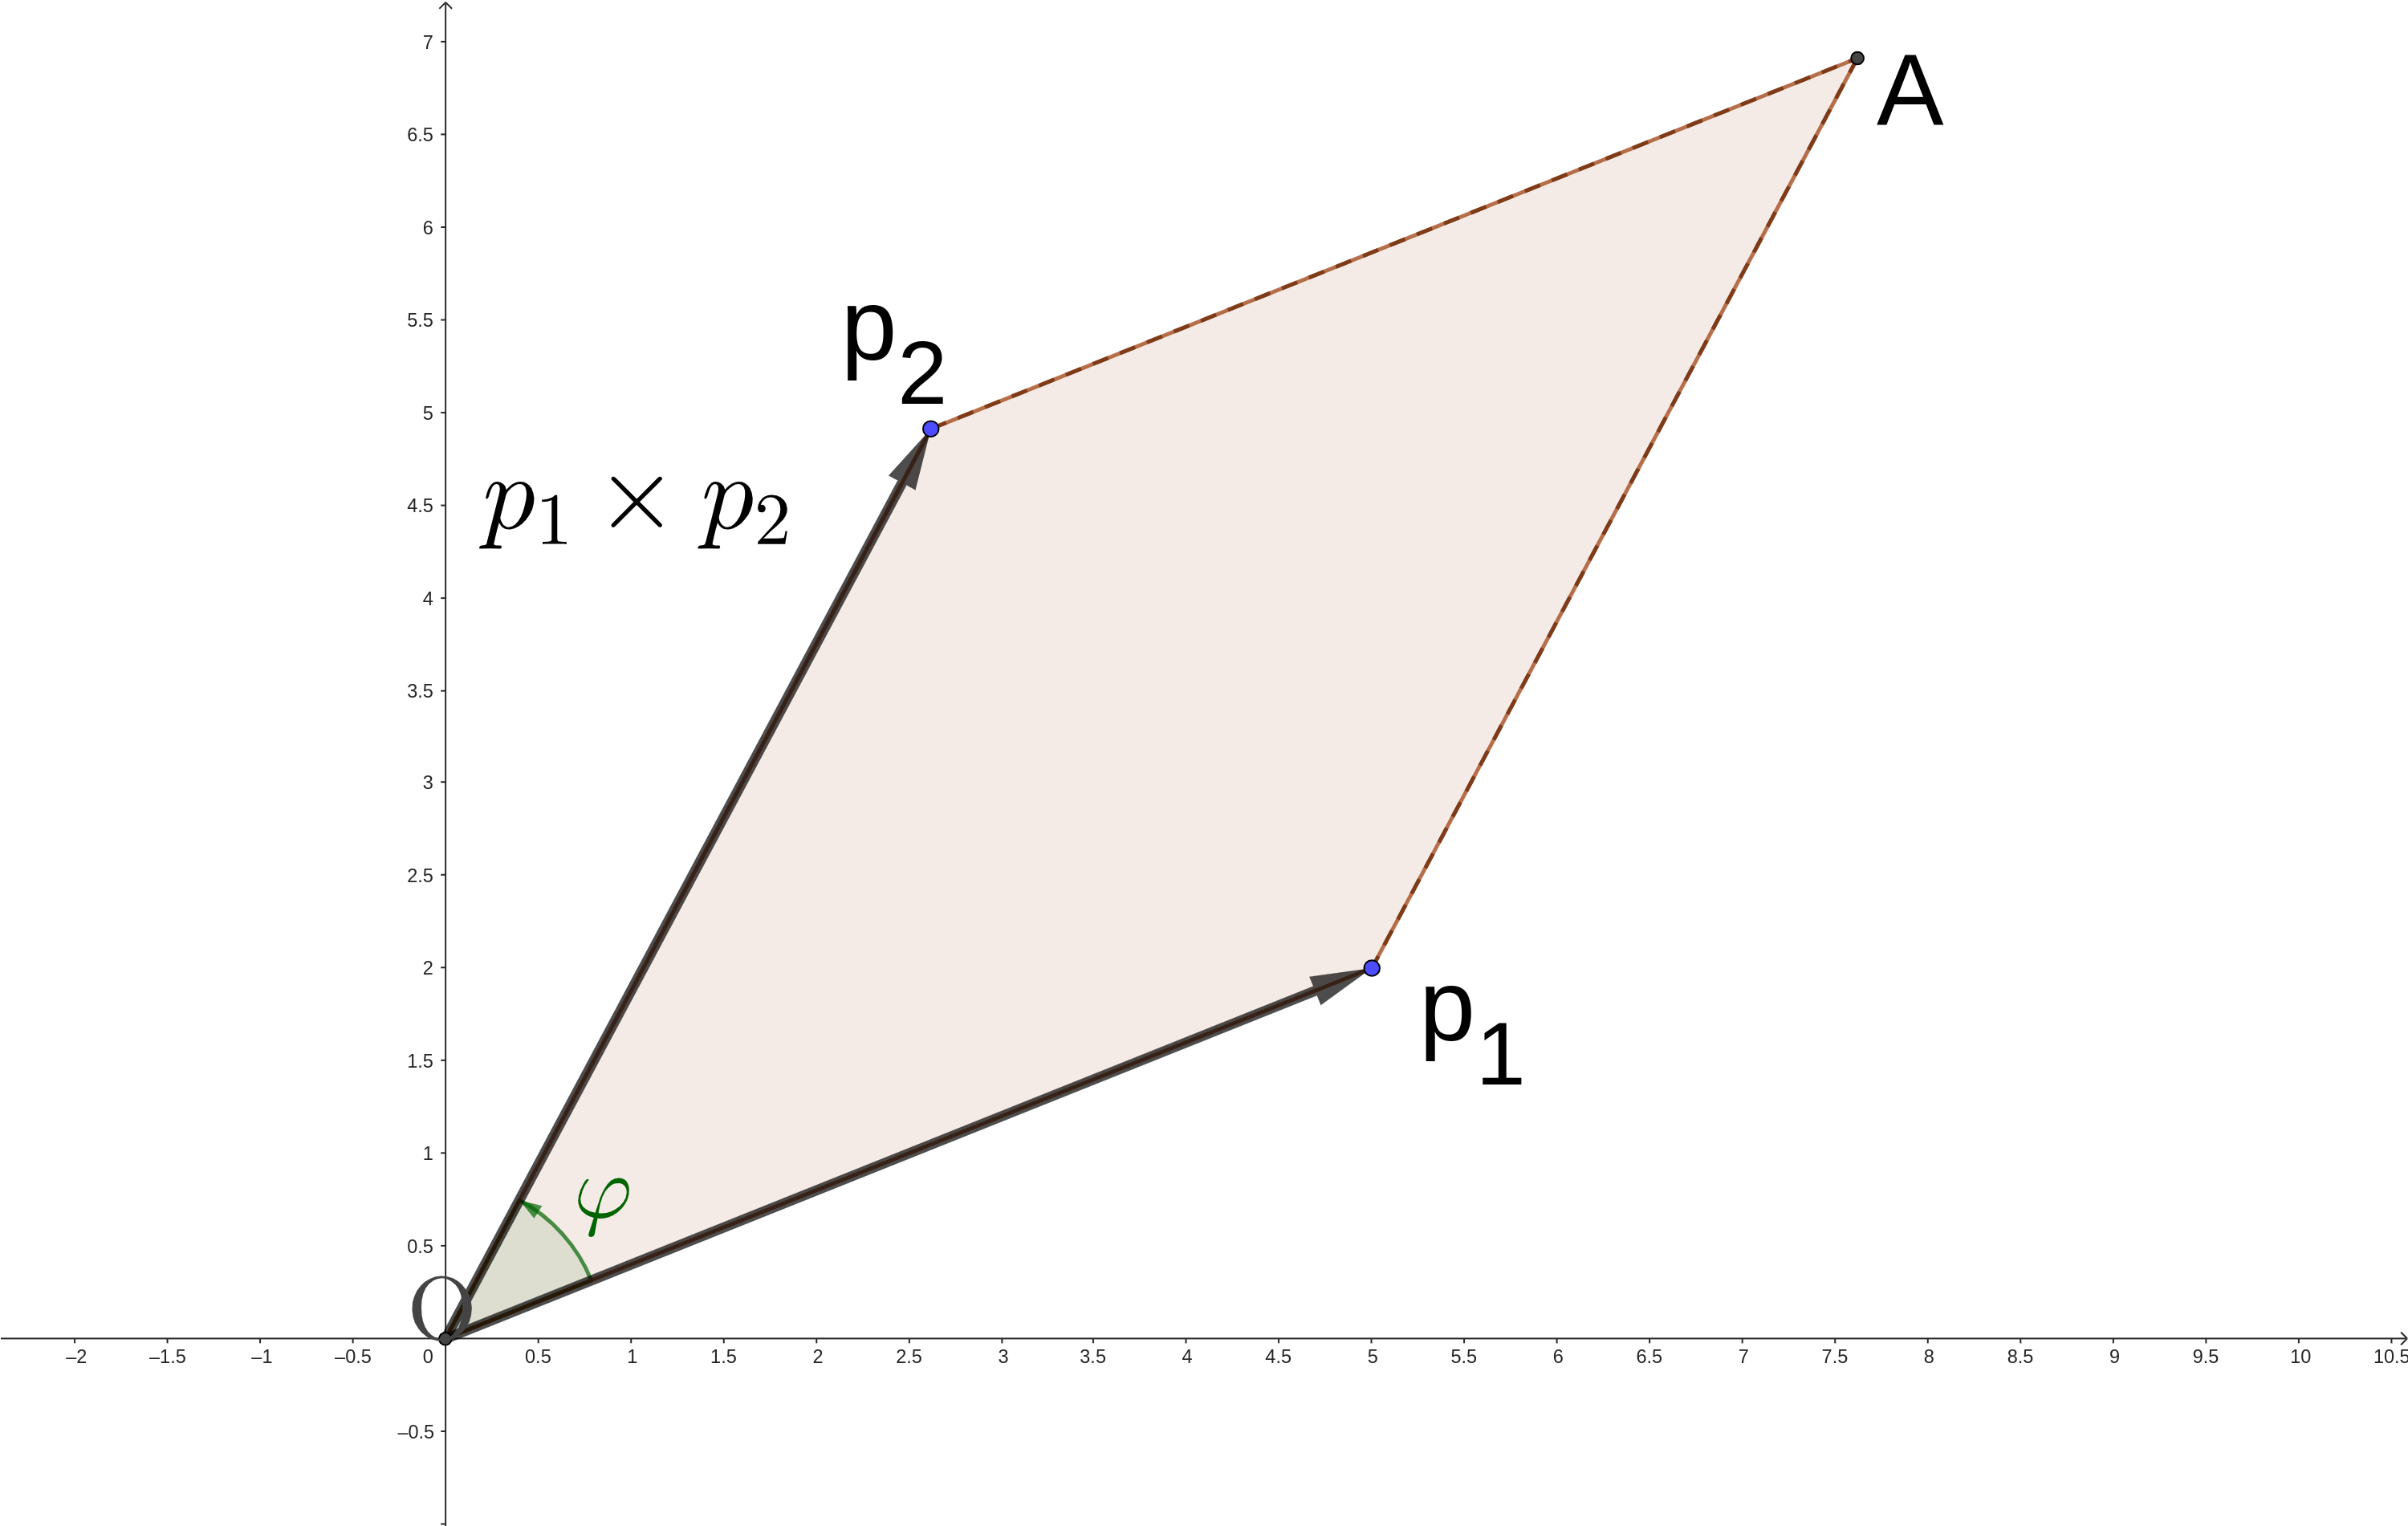
\includegraphics[scale = 0.6]{geogebra-export.png}
    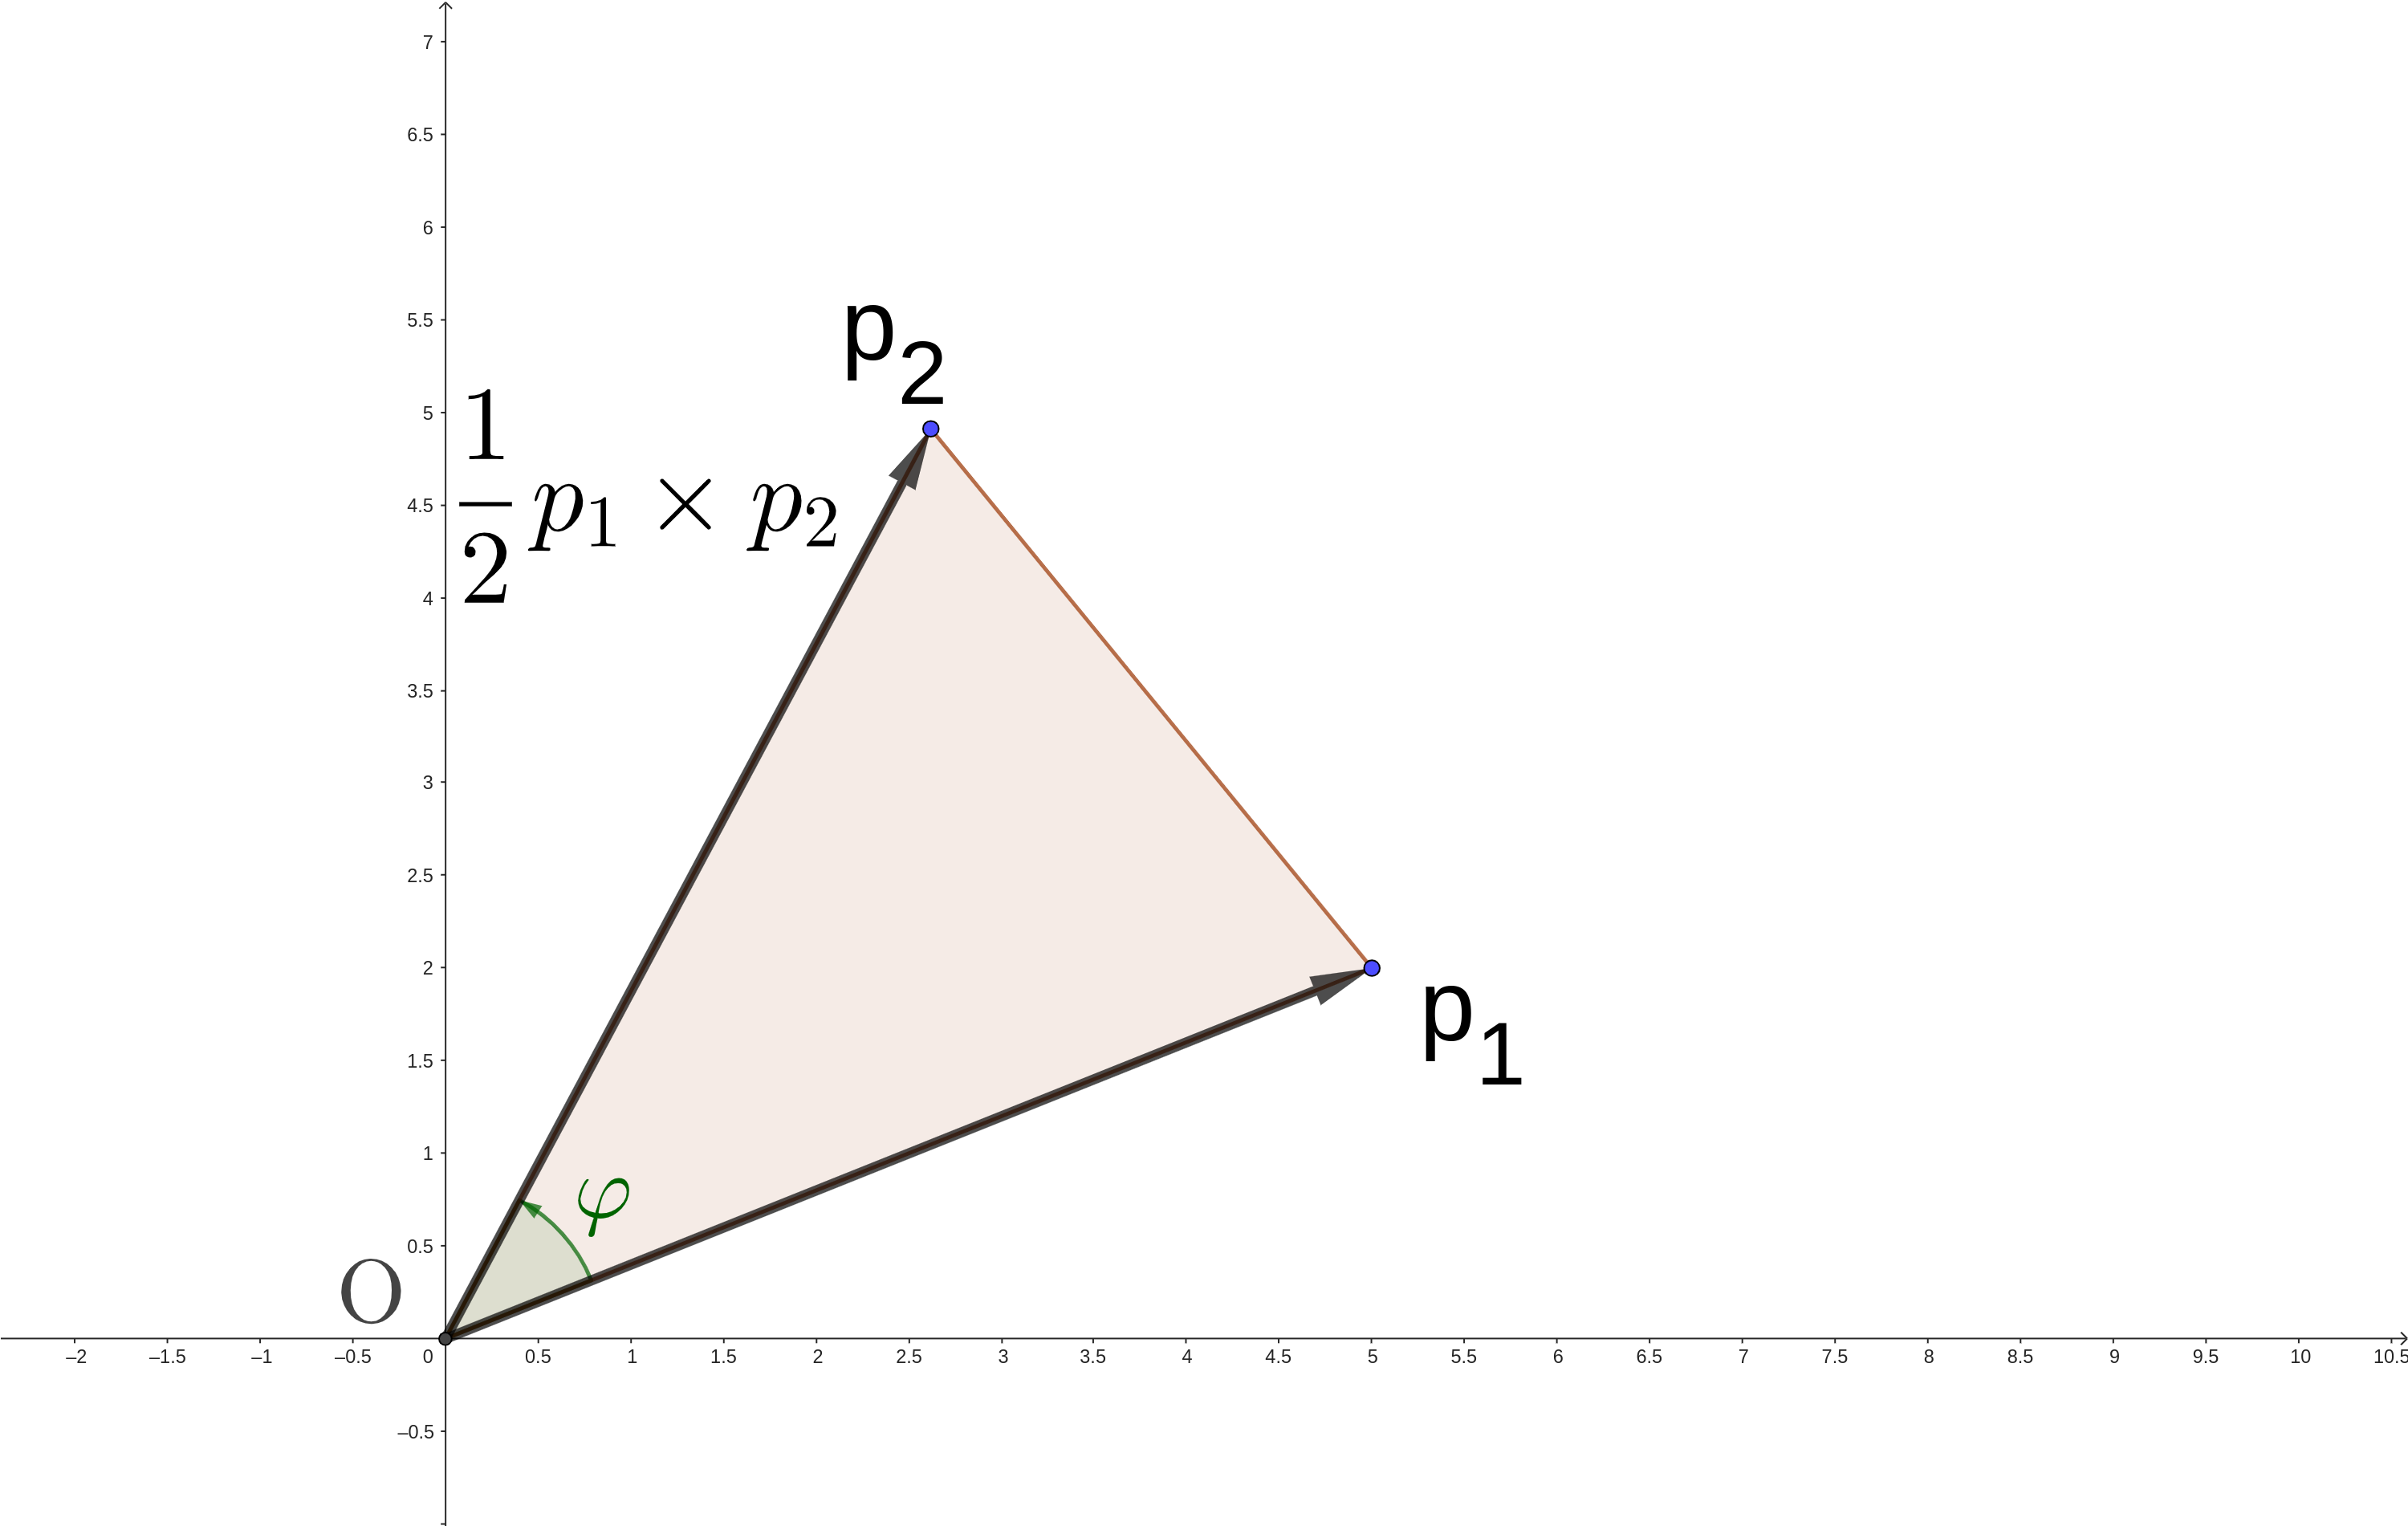
\includegraphics[scale =0.6]{geogebra-export1.png}
\end{figure}
Άρα το $\frac{1}{2}\bf p_1 \times p_2$ εκφράζει το προσημασμένο εμβαδό του τριγώνου $\bf Op_1p_2$ ($E(\bf Op_1p_2)$)(βλ. πάνω σχήμα δεξιά)\\

Έστώ τα σημεία $p_1,p_2,p_3$ το παρακάτατω σχήματος
\begin{figure}[H]

    \centering
    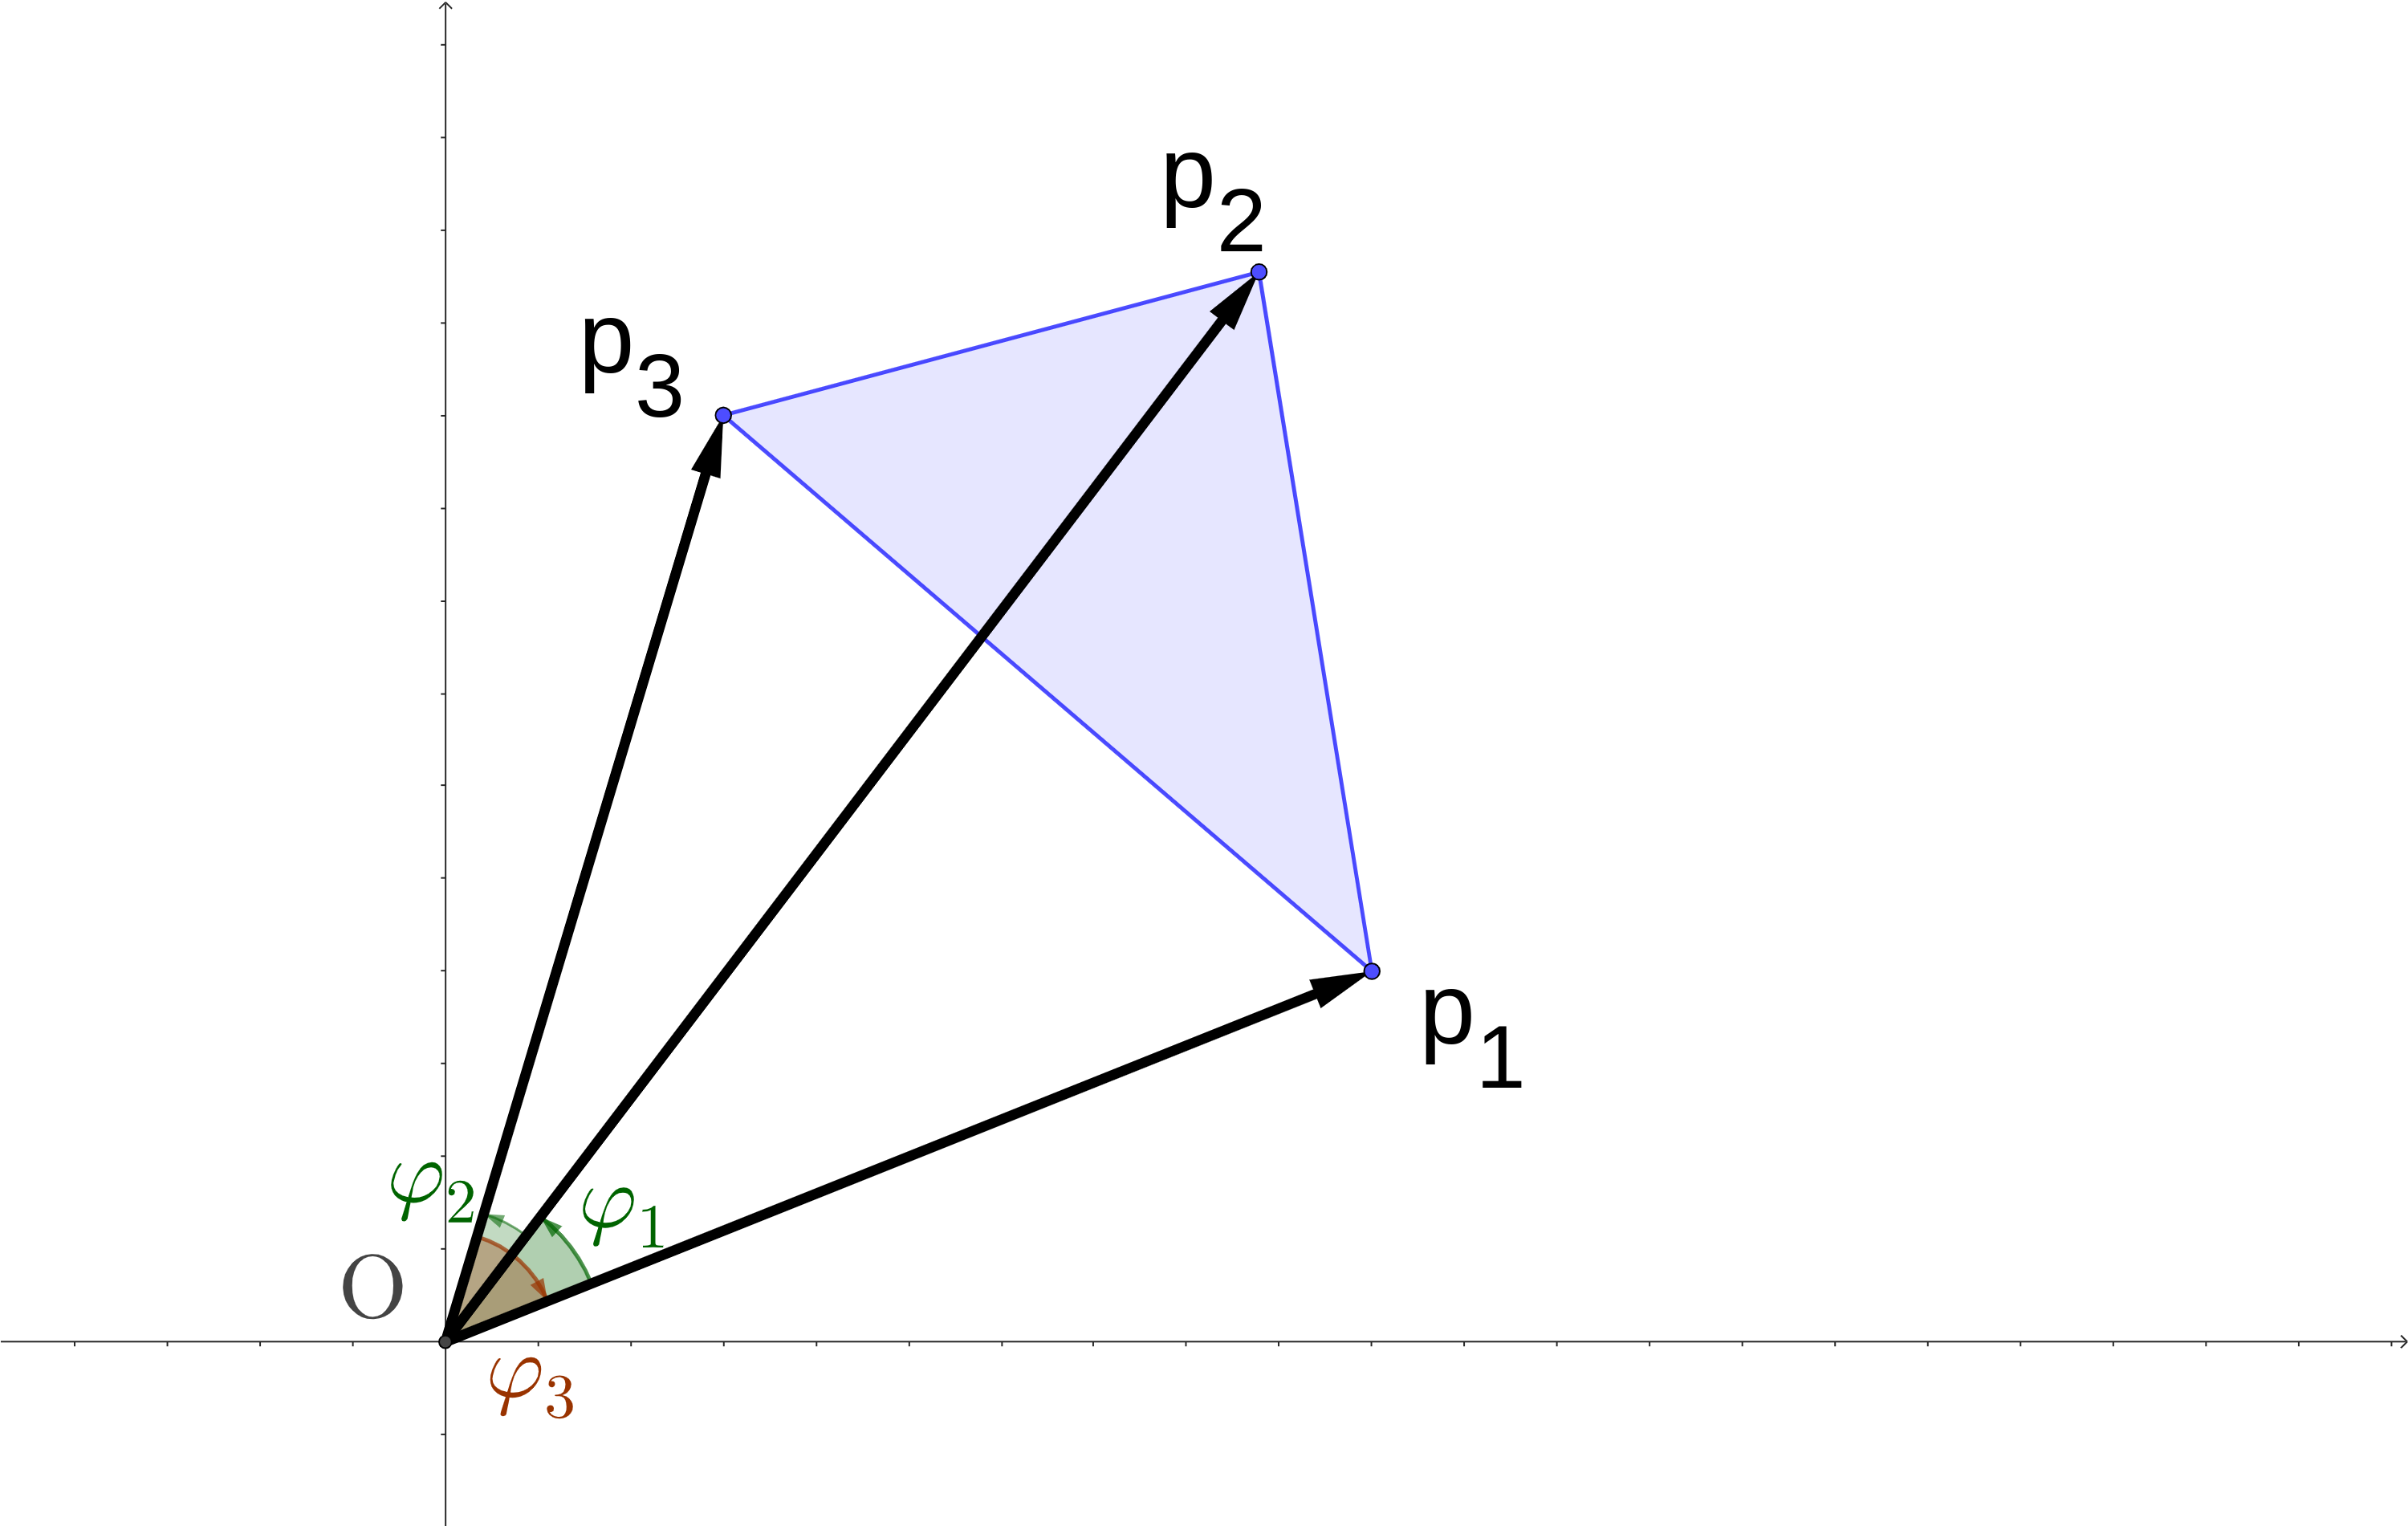
\includegraphics[scale = 1]{geogebra-export3.png}
\end{figure}
Έχουμε οτι :
\begin{itemize}
    \item $\frac{1}{2}p_1\times p_2 = |E({\bf Op_1p_2})|>0$ διότι η γωνία $\phi_1$ είναι αριστερόστροφη
    \item $\frac{1}{2}p_2\times p_3 = |E({\bf Op_2p_3})|>0$ διότι η γωνία $\phi_2$ είναι αριστερόστροφη
    \item $\frac{1}{2}p_3\times p_1 = -|E({\bf Op_3p_1})|<0$ διότι η γωνία $\phi_3$ είναι δεξιόστροφή
\end{itemize}

Άρα  
\begin{align*}
    \frac{1}{2}\sum_{i=1}^3 p_i\times p_{i+1} &=\frac{1}{2}(p_1\times p_2 + p_2\times p_3+ p_3\times p_1) =\\
    &=  |E({\bf Op_1p_2})| + |E({\bf Op_2p_3})| -|E({\bf Op_3p_1})| =E({\bf p_1p_2p_3}) 
\end{align*}
Άρα επιβεβαιώνεται ο τύπος \textlatin{Meister-Gauss} για τρία σημεία. Θα αποδείξουμε μέσω επαγωγής οτι ισχύει και για $n>3$ σημεία.\\
Έστω οτι ισχυεί για $n=k$ σημειά, δηλαδή $E_k =  \frac{1}{2}\sum_{i=0}^{k-1} p_i\times p_{i+1}$ με $p_k = p_0$. Tότε αρκει να δείξουμε οτι αν προσθέσουμε ένα ακομα σήμειο $\bf p_{k}$ θα ισχύει $E_{k+1} =  \frac{1}{2}\sum_{i=0}^{k} p_i\times p_{i+1}$ με $p_{k+1} = p_0$

\begin{figure}[H]

    \centering
    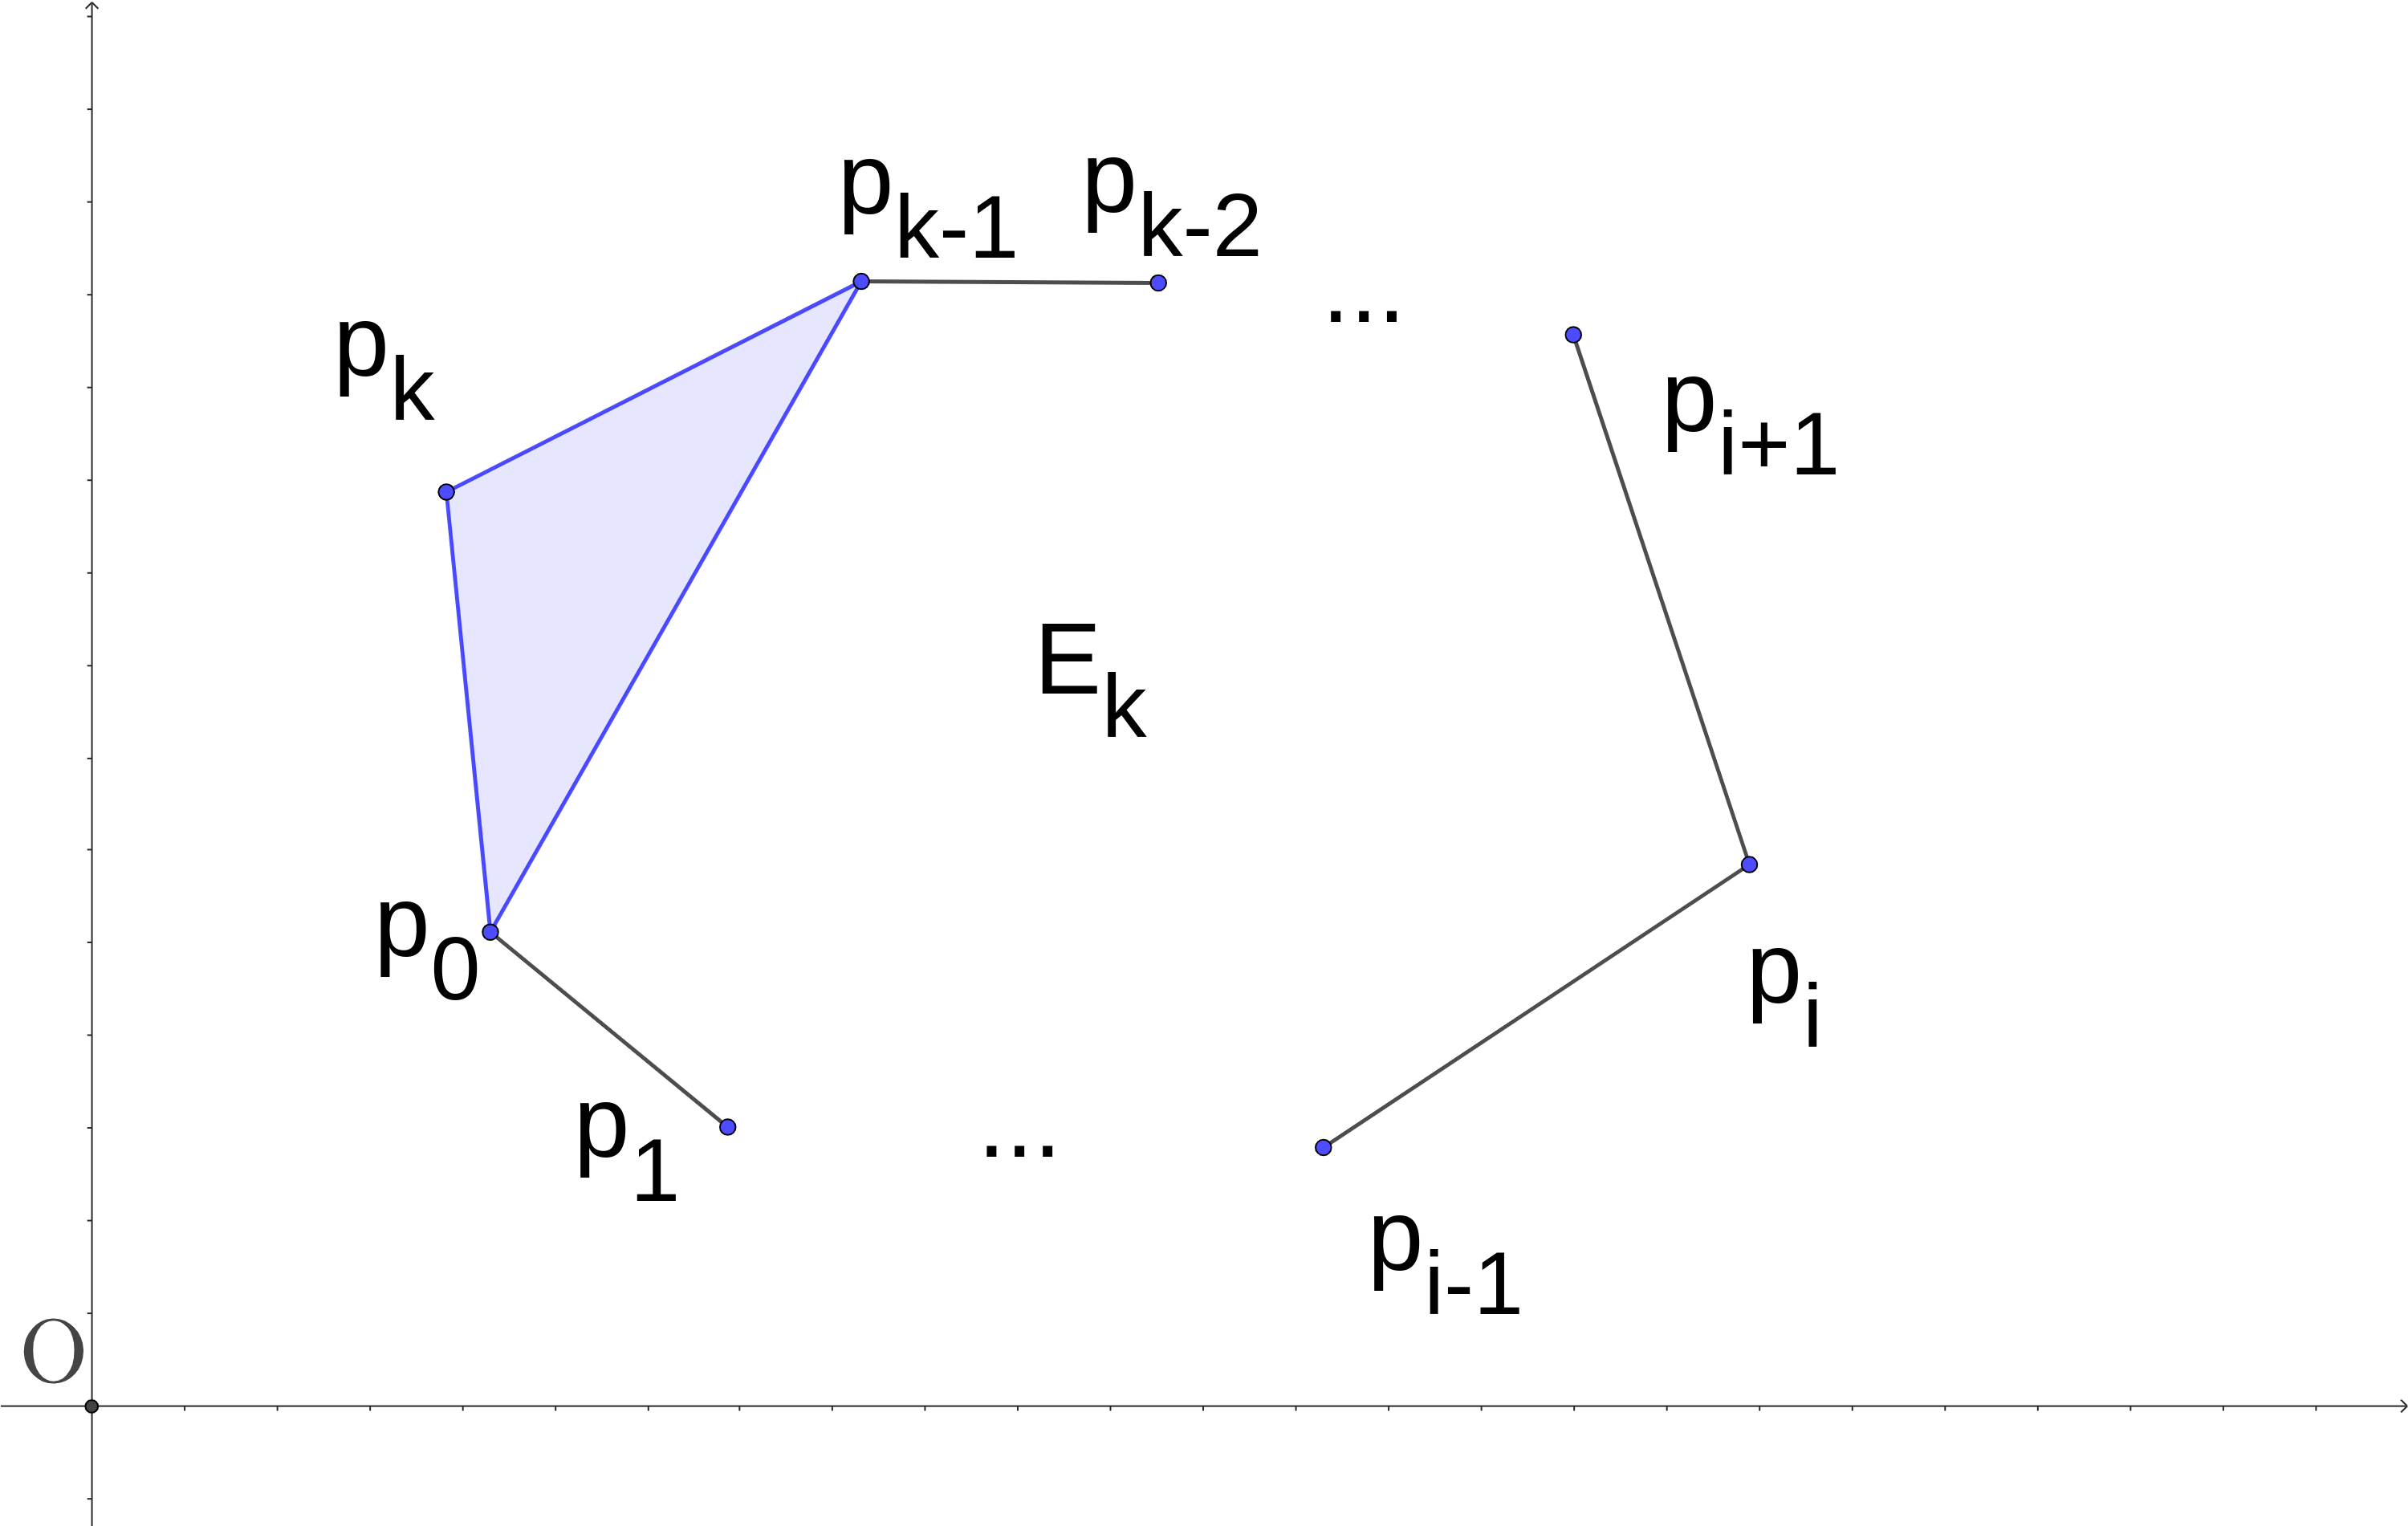
\includegraphics[scale = 1]{geogebra-export4.png}
\end{figure}
Βλέπουμε απο το παραπάνω σχήμα οτι 
\begin{align*}
    E_{k+1} &= E_k + E({\bf p_{k-1}p_{k}p_0}) =\\
    &=  \frac{1}{2}\sum_{i=0}^{k-1} p_i\times p_{i+1} + \frac{1}{2} (p_{k-1}\times p_{k} + p_{k}\times p_{0} + p_0\times p_{k-1}) = \\
    &=  \frac{1}{2}\sum_{i=0}^{k-2} p_i\times p_{i+1} + \cancelto{0}{\frac{1}{2}p_{k-1}\times p_{0}+ \frac{1}{2}p_0\times p_{k-1}}+\frac{1}{2} (p_{k-1}\times p_{k} + p_{k}\times p_{0} ) = \\
    &=  \frac{1}{2}\sum_{i=0}^{k-2} p_i\times p_{i+1}+\frac{1}{2} (p_{k-1}\times p_{k} + p_{k}\times p_{0} ) =\frac{1}{2}\sum_{i=0}^{k} p_i\times p_{i+1}
\end{align*}
Επομένως ισχυεί για $n=k+1$ και άρα ισχύει για κάθε $n\geq 3$\\
\rule{\textwidth}{.5pt}
\section*{Άσκηση 2}


Aρχικά παρατηρούμε οτι σε ένα κανονικό πολύεδρο, το γινόμενο του πλήθους το εδρών ($F$) με τον αριθμό των ακμών που περιβάλουν μια εδρα ($n$) είναι ίσο με το 
διπλάσιο τουν συνολικού αριθμού ακμών του πολυέδρου ($E$) δηλαδή $nF=2E$. O λόγος είναι οτι όταν παίρνουμε το γίνόμενο $nF$ οι κοίνες ακμές για δύο γειτονικές έδρες πρoσμετρούνται δύο φορές.
Επίσης ισχύει οτι o αριθμός των ακμών που συντρέχουν σε ένα κόμβο ($m$) επί τον αριθμό των κόμβων ($V$) είναι πάλι ίσο με $2E$ καθώς οι ακμές που ενώνουν δύο γειτονικόυς κόμβους  πρoσμετρούνται δύο φορές.
Άρα καταλήγουμε με την σχέση 
$$nF = mV =2E  \Rightarrow F = \frac{2E}{n},\; V = \frac{2E}{m}$$
Αντικαθιστώντας στο τύπο του ευκλείδη παίρνουμε
$$
    V-E+F=2 \Leftrightarrow \frac{2E}{n} -E + \frac{2E}{m} =2 \Leftrightarrow \frac{2}{n} -1 + \frac{2}{m} =\frac{2}{E} \Leftrightarrow \frac{1}{n} + \frac{1}{m} =\frac{1}{2}+\frac{1}{E}
$$
$$\xRightarrow{E>0}\frac{1}{n} + \frac{1}{m} >\frac{1}{2}$$
Για να υπάρχει μια έδρα πρέπει υποχρεωτικά $n\geq 3$ και για να υπάρχει το πολύεδρο πρεπει υποχρεωτικά $m\geq 3$. Άρα τα ζευγάρια $(n,m)$ που ικανοποιούν την παραπάνω ανισότητα είναι:
\begin{enumerate}
    \item $n=3$ και $m=3$: Η κάθε έδρα είναι ένα ισόπλευρο τρίγωνο και σε κάθε κόμβο συναντώνται τρείς έδρες (Τετράεδρο)
    \item $n=3$ και $m=4$: Η κάθε έδρα είναι ένα ισόπλευρο τρίγωνο και σε κάθε κόμβο συναντώνται τέσσερις έδρες (Οκτάεδρο)
    \item $n=3$ και $m=5$: Η κάθε έδρα είναι ένα ισόπλευρο τρίγωνο και σε κάθε κόμβο συναντώνται πέντε έδρες (Είκοσαεδρο)
    \item $n=4$ και $m=3$: Η κάθε έδρα είναι ένα τετράγωνο και σε κάθε κόμβο συναντώνται τρείς έδρες (Κύβος)
    \item $n=5$ και $m=3$: Η κάθε έδρα είναι ένα πεντάγωνο και σε κάθε κόμβο συναντώνται τρείς έδρες (Δωδεκάεδρο)
\end{enumerate}

Άρα σύνολο πέντε κανονικά πολύεδρα\\
\rule{\textwidth}{.5pt}
\section*{Άσκηση 3}
{\bf Για το πλήθος των διαγωνίων}:\\
Απο ένα κόμβο μπορουν να προκύψουν διαγώνιοι με όλους του άλλους κόμβους πλήν του εαυτού του και των δύο γειτόνων του, άρα $n-3$ διαγώνιοι. Για $n$ κόμβους υπάρχουν $n(n-3)$ διαγώνιοι. Παρατηρούμε οτι το πληθος των διαγωνίων είναι ανεξάρτητο απο το αν είναι συνεκτικό το πολύγονο ή απο το αν εχεί τρύπες.\\ \\
{\bf Για το πλήθος τών τριγώνων}:\\
Έστω οτι η μή συνεκτική περιοχή αποτελείται απο $p$ συνεκτικές περιοχές. Για την συνεκτική περιοχή $i$ ($1\leq i\leq p$) ορίζουμε $h_i$ το πλήθος τών τρυπών τις και $n_i$ το πλήθος των κόμβων του συνόρου της. Ορίζουμε επίσης  $n_{i0}$ το πλήθος των κόμβων του εξωτερικού συνόρου της και  $n_{ij}$ το πλήθος των κόμβων της τρύπας $j$ ($1\leq j\leq h_i$)

Tο άθροισμα των εσωτερικών γωνιών του εξωτερικού συνόρου είναι $(n_{i0} -2 )180^o$ ενώ το άθροισμα των εξωτερικών γωνιών της τρύπας $j$ είναι $(n_{ij} +2 )180^o$. Αρα το άθροισμα των εσωτερικών γωνιών της συνεκτικής περιοχής $i$ είναι:
$$(n_{i0} -2 )180^o + \sum_{j=1}^{h_i}(n_{ij} +2 )180^o = \left(\sum_{j=0}^{h_i}n_{ij} +2 h_i - 2\right)180^o = \left(n_{i} +2 h_i - 2\right)180^o $$
Το άθροισμα των εσωτερικών γωνιών ενός τριγώνου είναι $180^o$ άρα  το πλήθος τών τριγώνων για τριγωνοποιήση της συνεκτικής περιοχής $i$ είναι 
$$T_i = \frac{\left(n_{i} +2 h_i - 2\right)180^o}{180^o} = n_{i} +2 h_i - 2$$
Άρα το πλήθος των τριγώνων για την τριγωνοποιήση της μή συνεκτικής περιοχής θα είναι το άθροισμα των τριγώνων της της κάθε συνεκτικής δηλαδή:
$$\sum_{i=1}^p T_i = \sum_{i=1}^p n_{i} +2 h_i - 2 =\sum_{i=1}^p n_{i}+ 2 \sum_{i=1}^p h_{i} -2p = n+2h - 2p$$
\rule{\textwidth}{.5pt}
\section*{Άσκηση 4}
Στο αποτέλεσμα της προηγούμενης άσκησης, αντικαθιστώντας με $p=1$ προκύπτει οτι το πλήθος τριγώνων της τριγωνοποιήσης για μια συνεκτική πολυγωνικη περιοχή με $n$ κόμβους και $h$ τρύπες είναι 
$n+2h - 2$. Γνωρίζουμε επίσης οτι σε ένα απλό πολύγωνο με $n$ κόμβους και τριγωνοποιήση $n-2$ τριγώνων, χρειάζονται το πολύ $\lfloor \frac{n}{3} \rfloor$ \textlatin{guards}. Άρα για πολύγωνο τριγωνοποιήσης $n+2h - 2$ τριγώνων, θα χρειάζονται
το πολύ $\lfloor \frac{n+2h}{3} \rfloor$ \textlatin{guards}\\
\rule{\textwidth}{.5pt}
\section*{Άσκηση 5}
O ζητούμενος αλγόριθμος είναι ο εξής:
\begin{enumerate}
    \item Αρχικά βρίσκουμε τα σημεία με την μέγιστη και ελαχιστη συνιστώσα στον κατακόρυφο άξονα $y_{max}$ και $y_{min}$ και υπολογίζουμε τις οριζόντιες ευθείες $h_{max}: y=y_{max}$ και $h_{min}: y=y_{min}$. H εύρεση τών $y_{max}$ και $y_{min}$
            μπόρει να γίνει σε χρόνο $O(n)$ με μια απλή αναζήτηση όλων των σημείων $p^{(i)}$ και βρίσκοντας το $\max_i\{p^{(i)}_y\}$ (και αντίστοιχα το $\min_i\{p^{(i)}_y\}$).
            \begin{figure}[H]

                \centering
                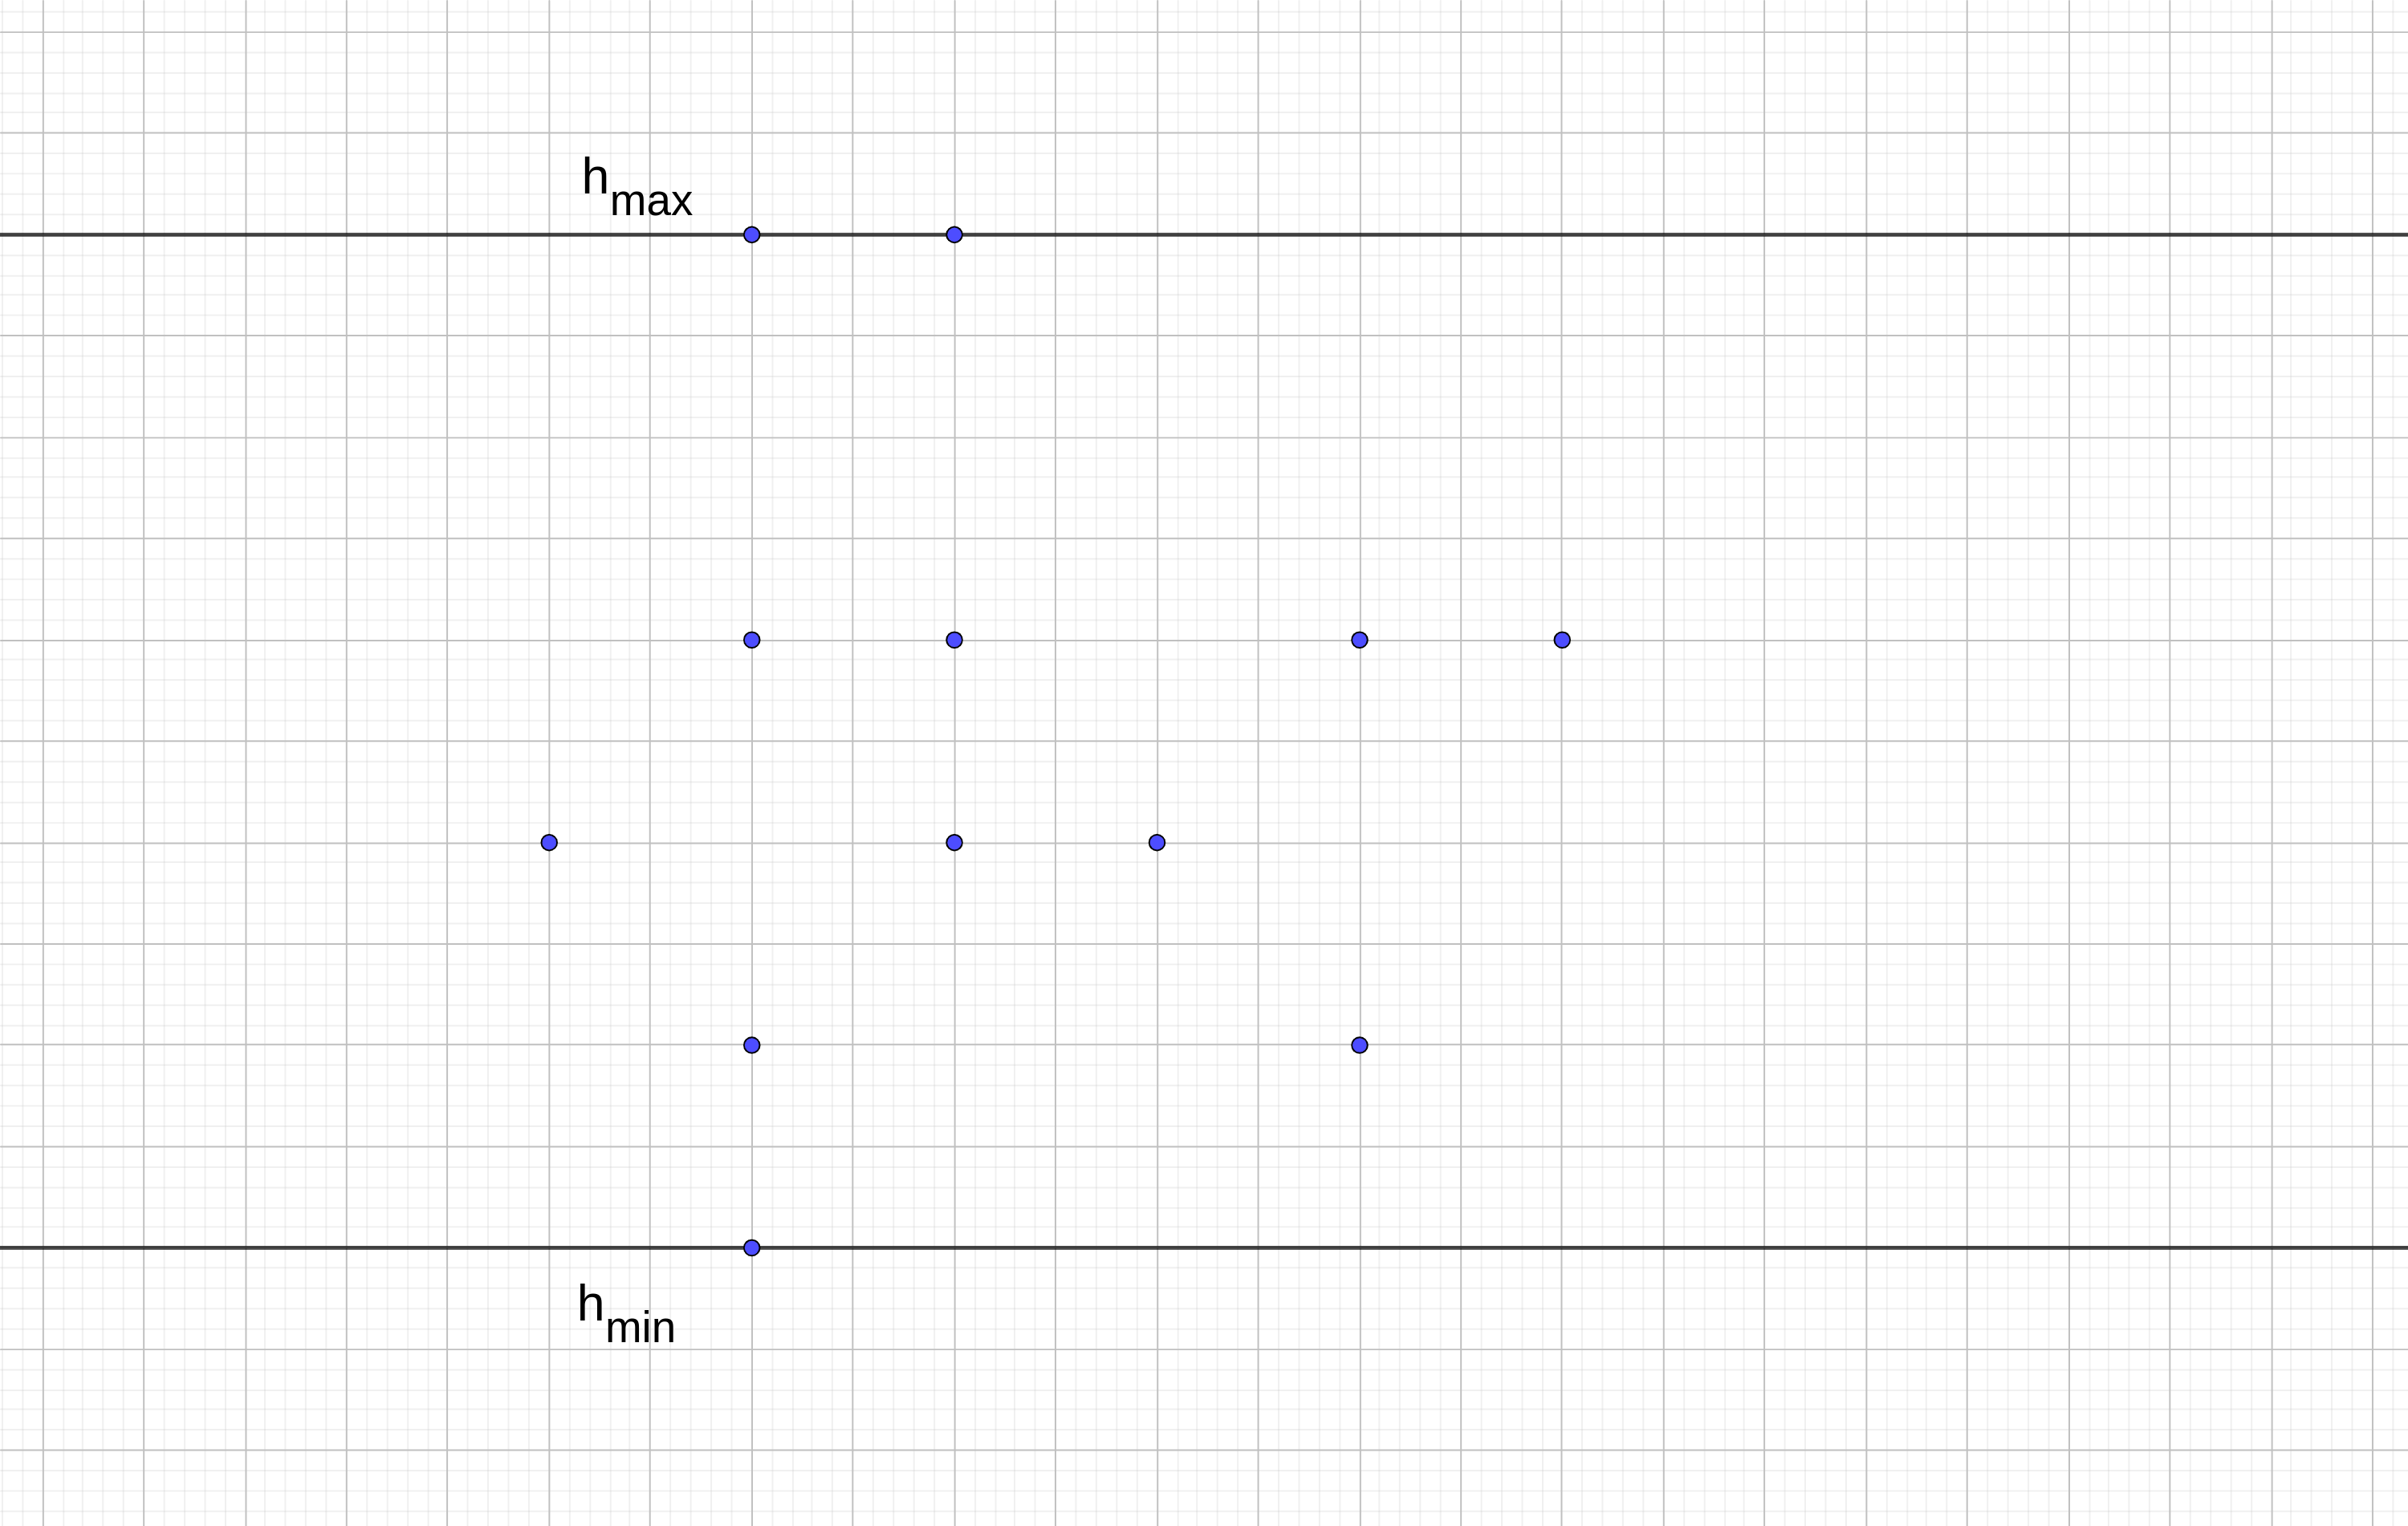
\includegraphics[scale = 0.8]{geogebra-export5.png}
            \end{figure}
    \item  Βρίσκουμε τα σημεία με την μέγιστη και ελαχιστη συνιστώσα στον οριζόντιο άξονα $x_{max}$ και $x_{min}$ και υπολογίζουμε τις κάθετες ευθείες $v_{max}: x=x_{max}$ και $v_{min}: x=x_{min}$. H εύρεση τών $x_{max}$ και $x_{min}$
    μπόρει να γίνει πάλι σε χρόνο $O(n)$ με αναζήτηση όλων των σημείων $p^{(i)}$ και βρίσκοντας το $\max_i\{p^{(i)}_x\}$ (και αντίστοιχα το $\min_i\{p^{(i)}_x\}$).
    \begin{figure}[H]

        \centering
        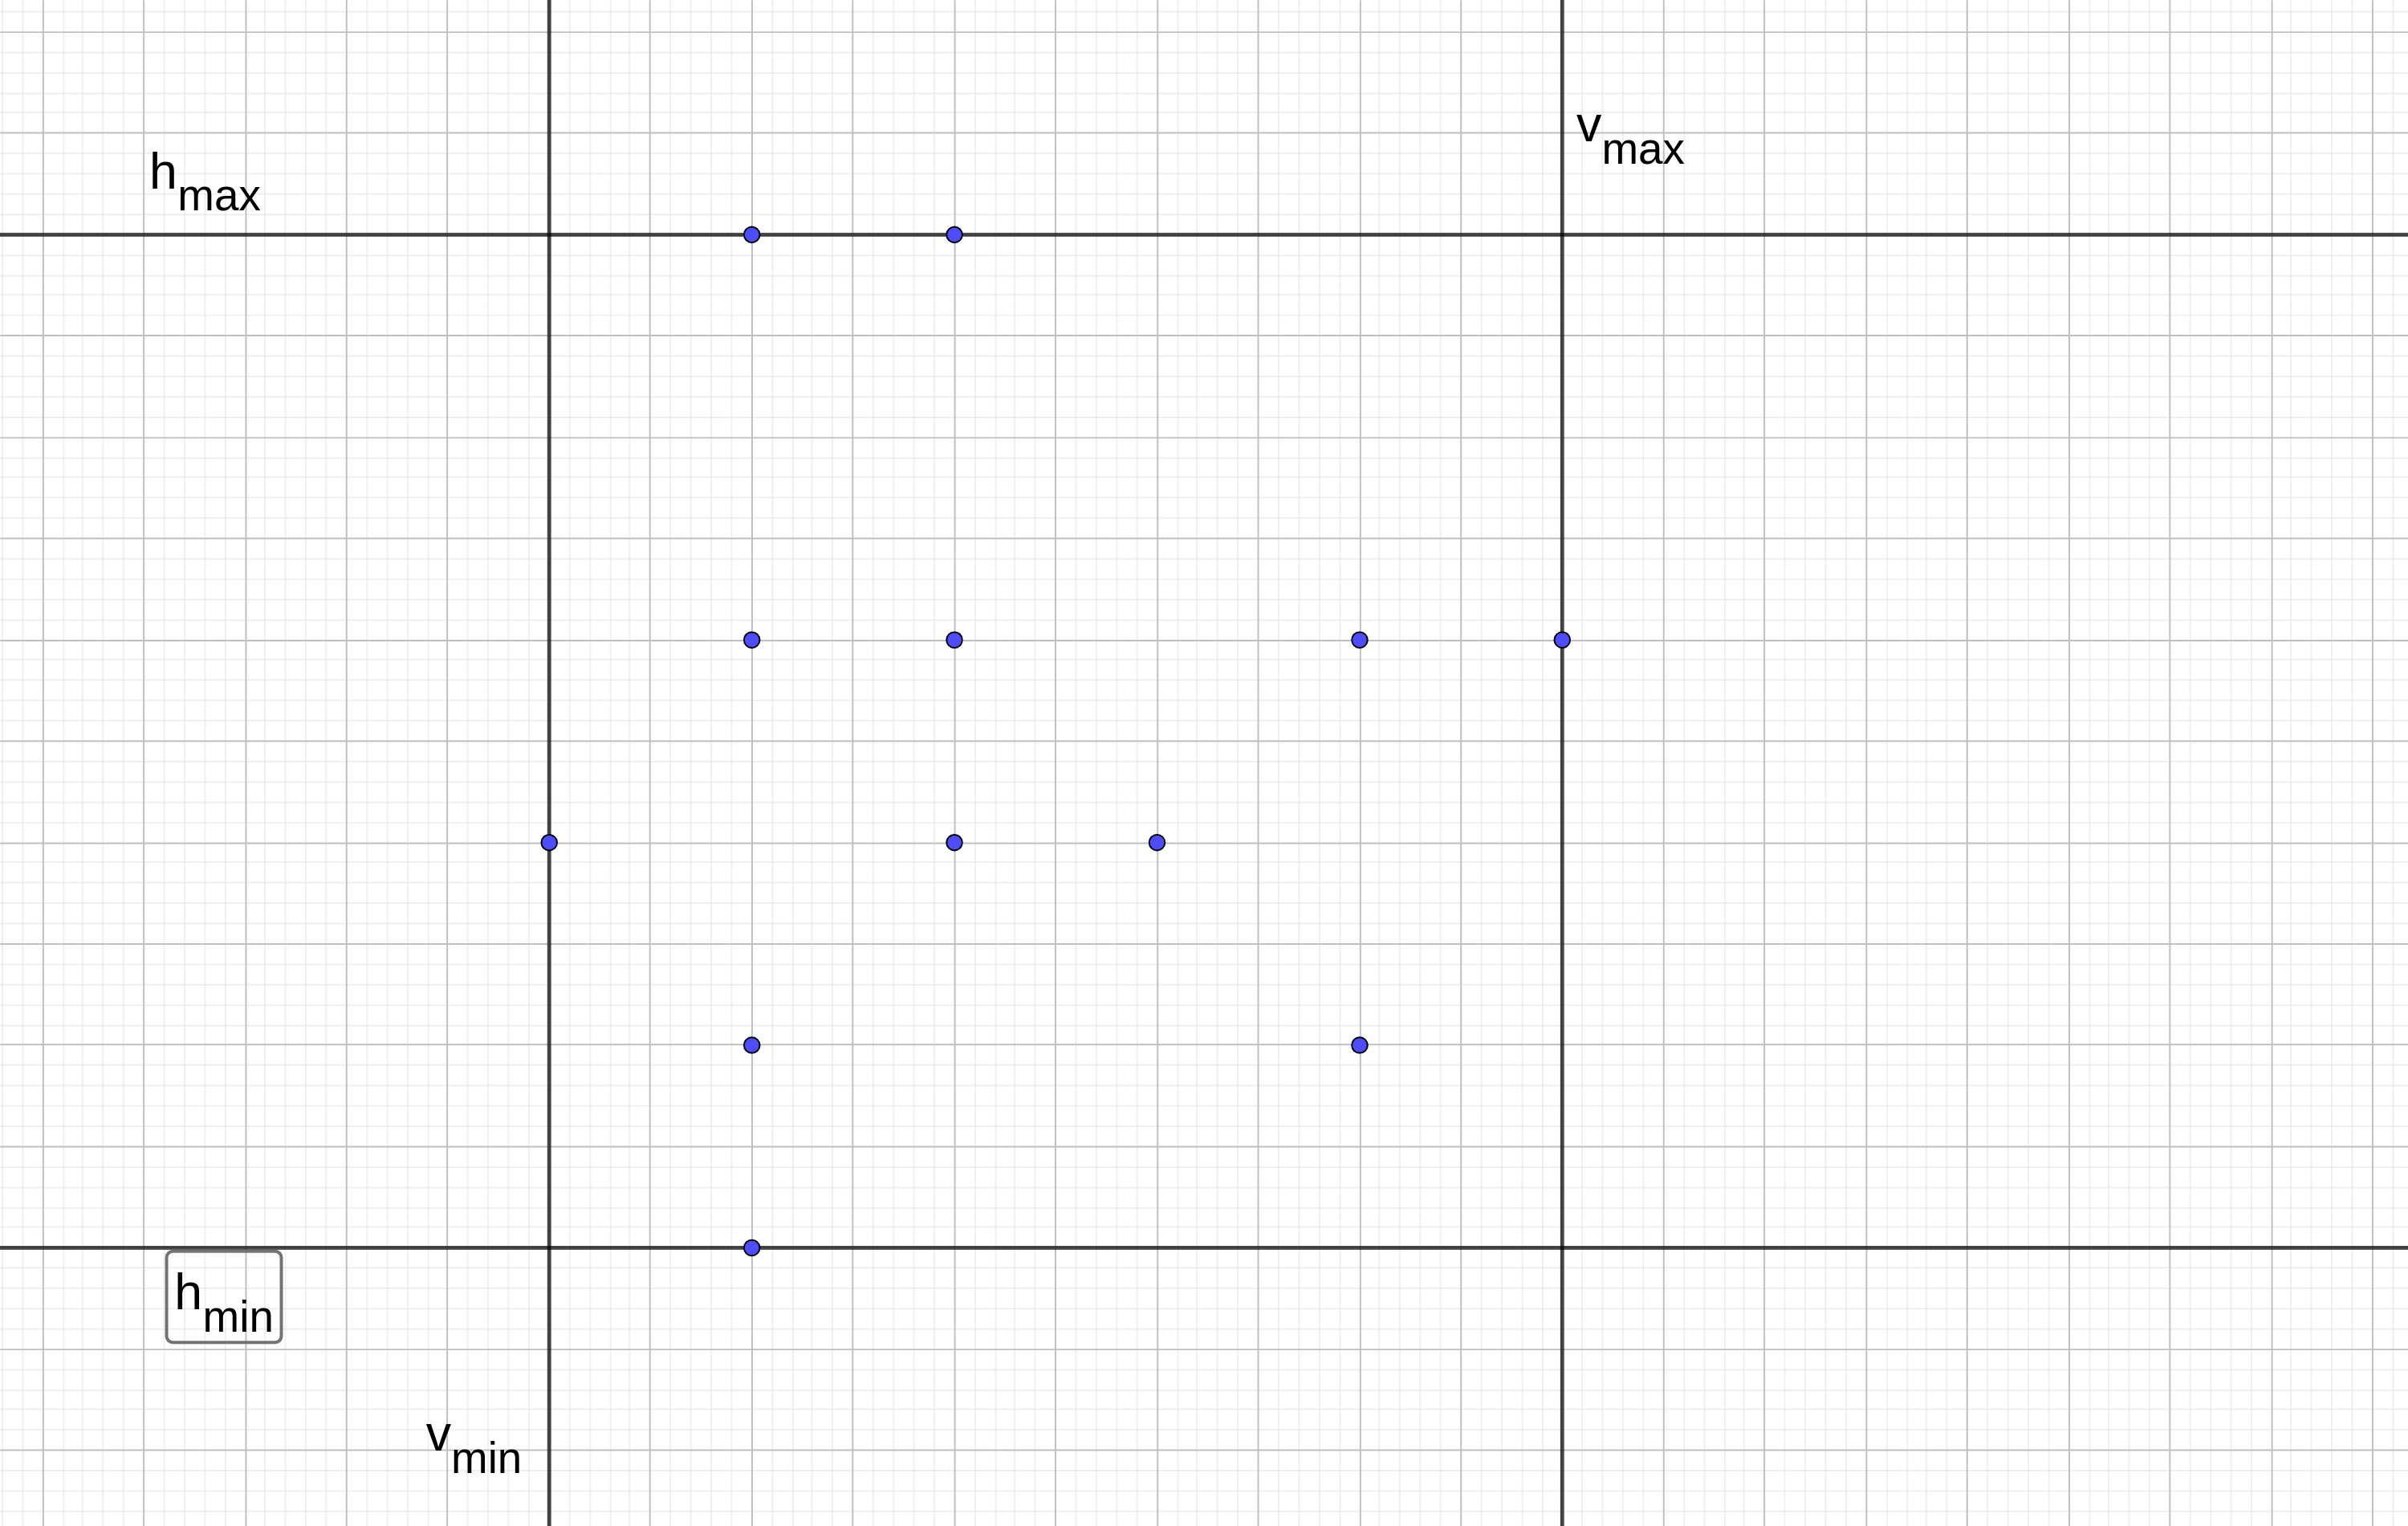
\includegraphics[scale = 0.8]{geogebra-export6.png}
    \end{figure}
    \item  Βρίσκουμε τα σημεία με την μέγιστη και ελαχιστη συνιστώσα στον άξονα $z_1$ με κλίση $+45^o$, $p^{z_{1(max)}}$ και $p^{z_{1(min)}}$ και υπολογίζουμε τις κάθετες  στον άξονα $z_1$ ευθείες $s_1^{max}: y=-x+(p^{z_{1(max)}}_y+p^{z_{1(max)}}_x)$ και 
    $s_1^{min}: y=-x+(p^{z_{1(min)}}_y+p^{z_{1(min)}}_x)$. O υπολογισμος των ευθειών $s_1^{max}$ και $s_1^{min}$
    μπόρει να γίνει σε χρόνο $O(n)$ με αναζήτηση όλων των σημείων $p^{(i)}$ και βρίσκοντας το $\max_i\{p^{(i)}_y+p^{(i)}_x\}$ (και αντίστοιχα το $\min_i\{p^{(i)}_y+p^{(i)}_x\}$).
    \begin{figure}[H]

        \centering
        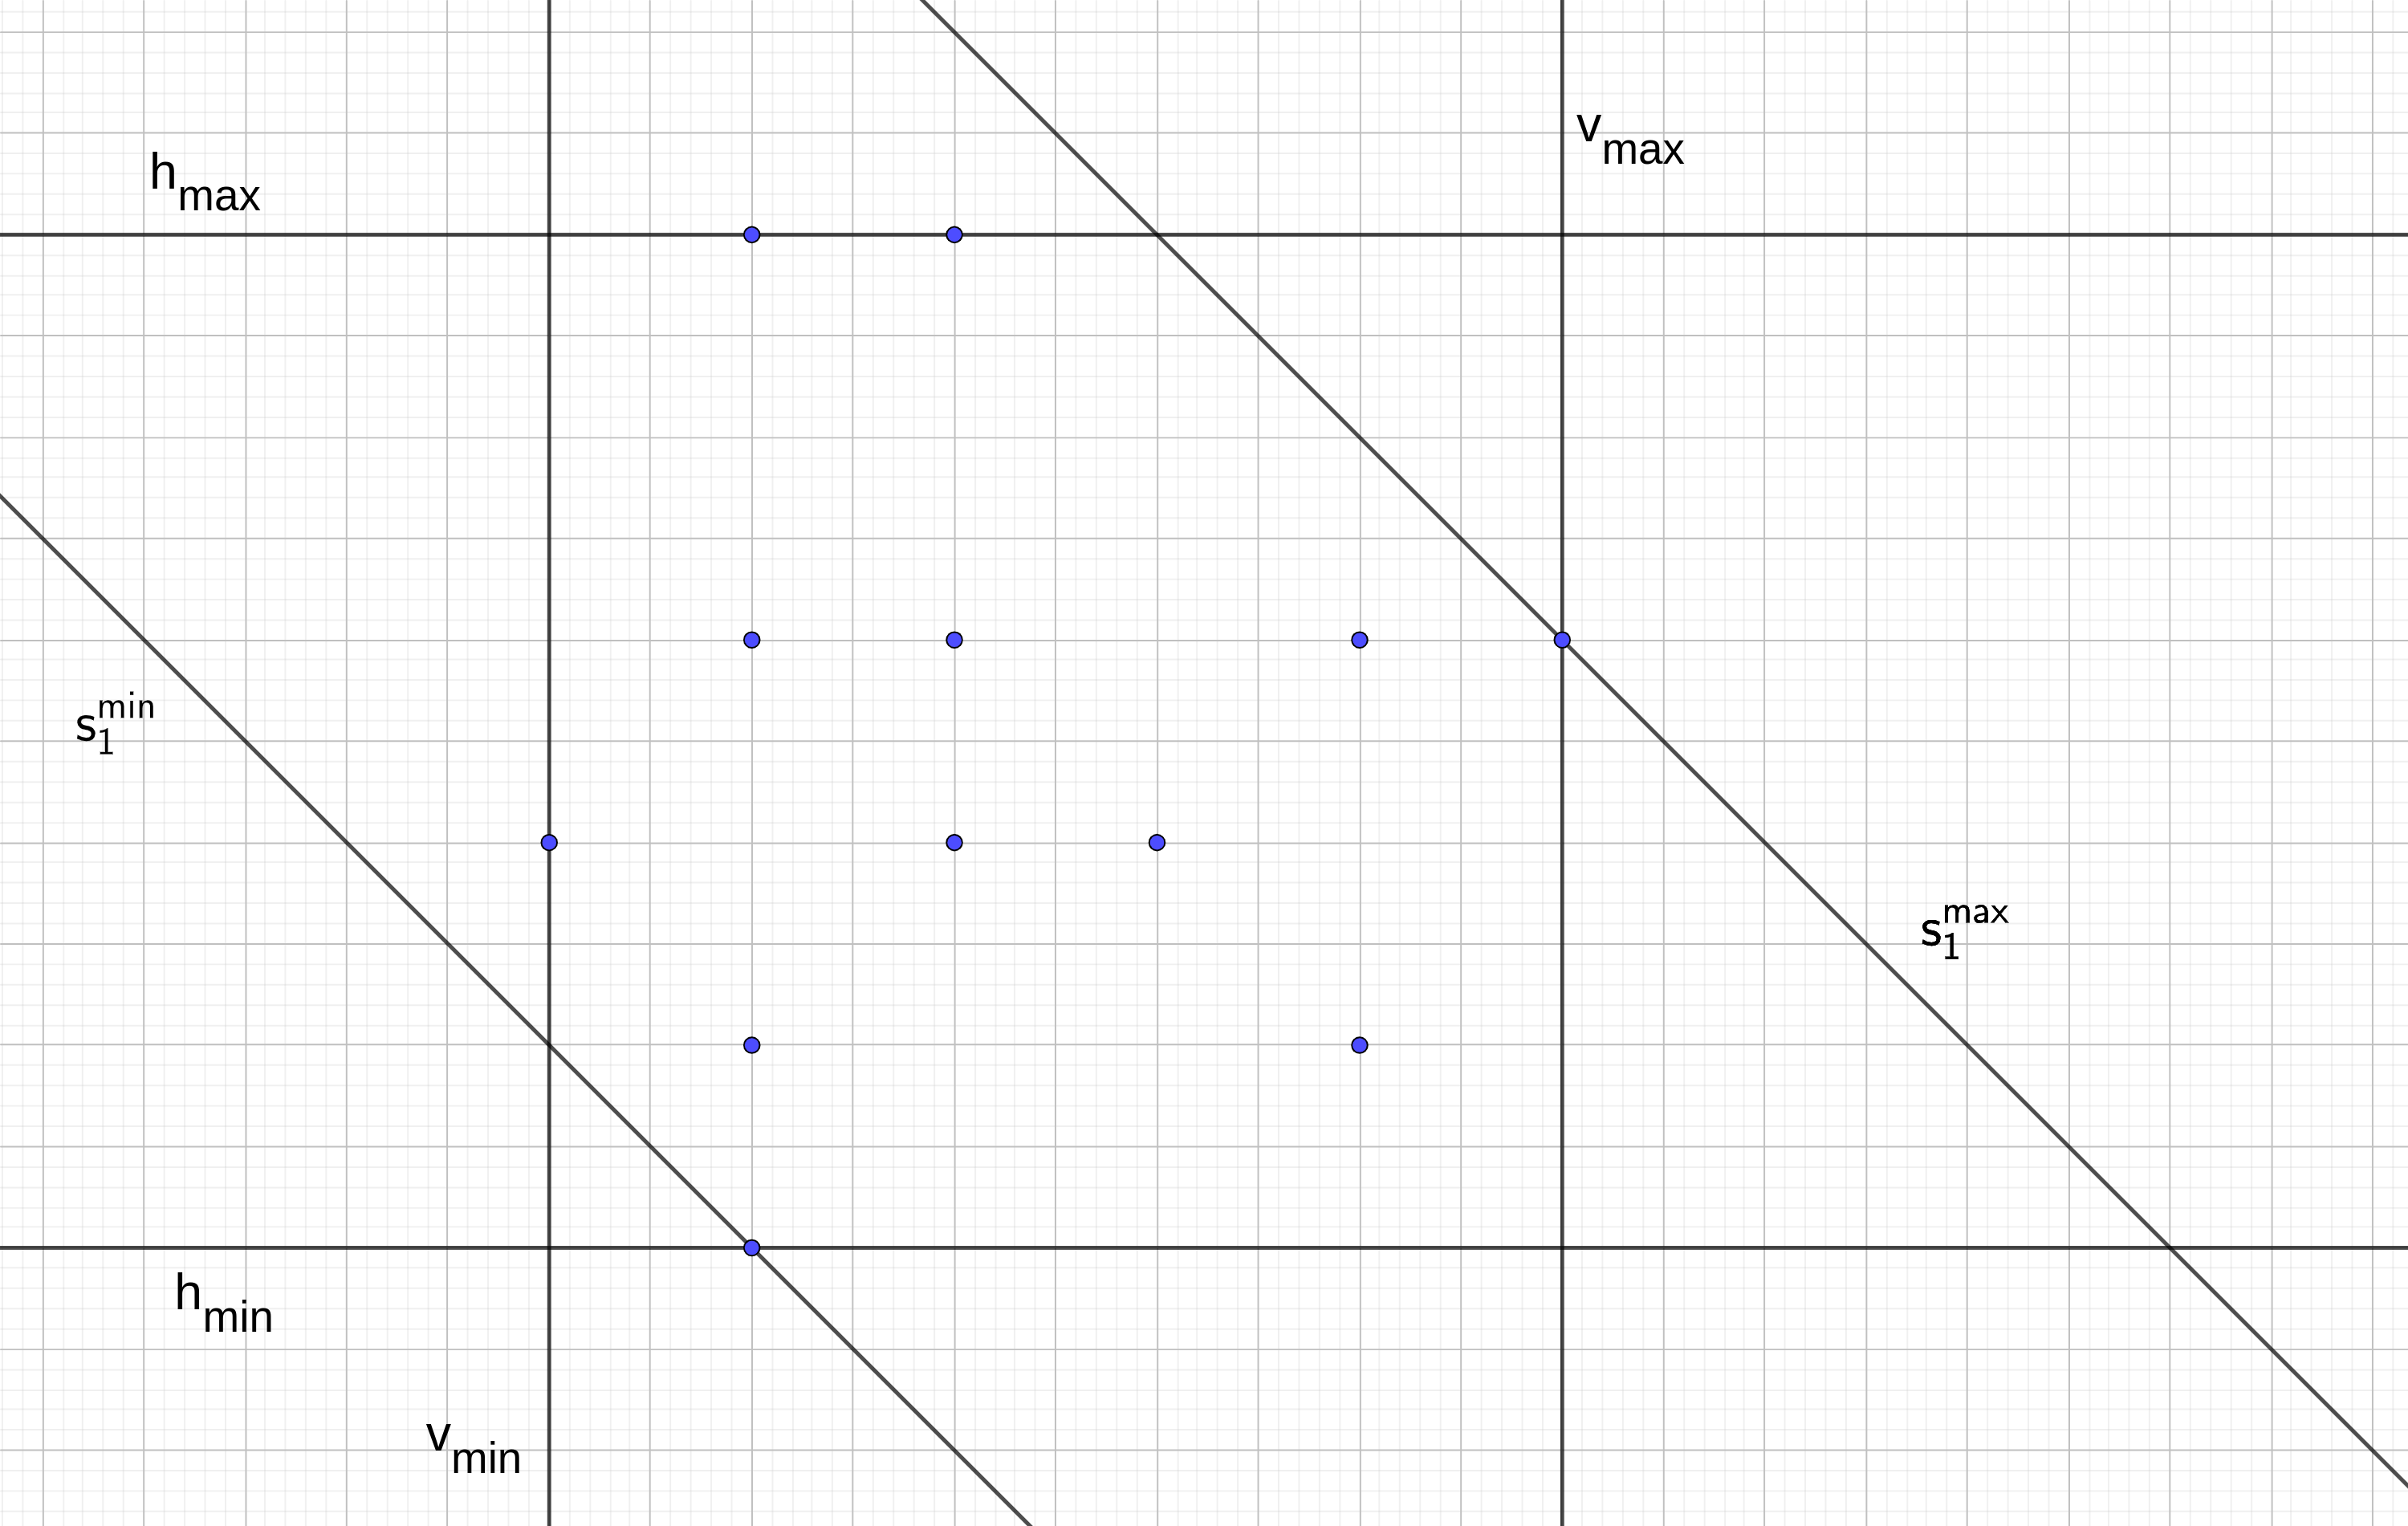
\includegraphics[scale = 0.8]{geogebra-export7.png}
    \end{figure}
    \item  Βρίσκουμε τα σημεία με την μέγιστη και ελαχιστη συνιστώσα στον άξονα $z_2$ με κλίση $-45^o$, $p^{z_{2(max)}}$ και $p^{z_{2(min)}}$ και υπολογίζουμε τις κάθετες  στον άξονα $z_2$ ευθείες $s_2^{max}: y=x+(p^{z_{2(max)}}_y-p^{z_{2(max)}}_x)$ και 
    $s_2^{min}: y=x+(p^{z_{2(min)}}_y-p^{z_{2(min)}}_x)$. O υπολογισμος των ευθειών $s_2^{max}$ και $s_2^{min}$
    μπόρει να γίνει σε χρόνο $O(n)$ με αναζήτηση όλων των σημείων $p^{(i)}$ και βρίσκοντας το $\max_i\{p^{(i)}_y-p^{(i)}_x\}$ (και αντίστοιχα το $\min_i\{p^{(i)}_y-p^{(i)}_x\}$).
    \begin{figure}[H]

        \centering
        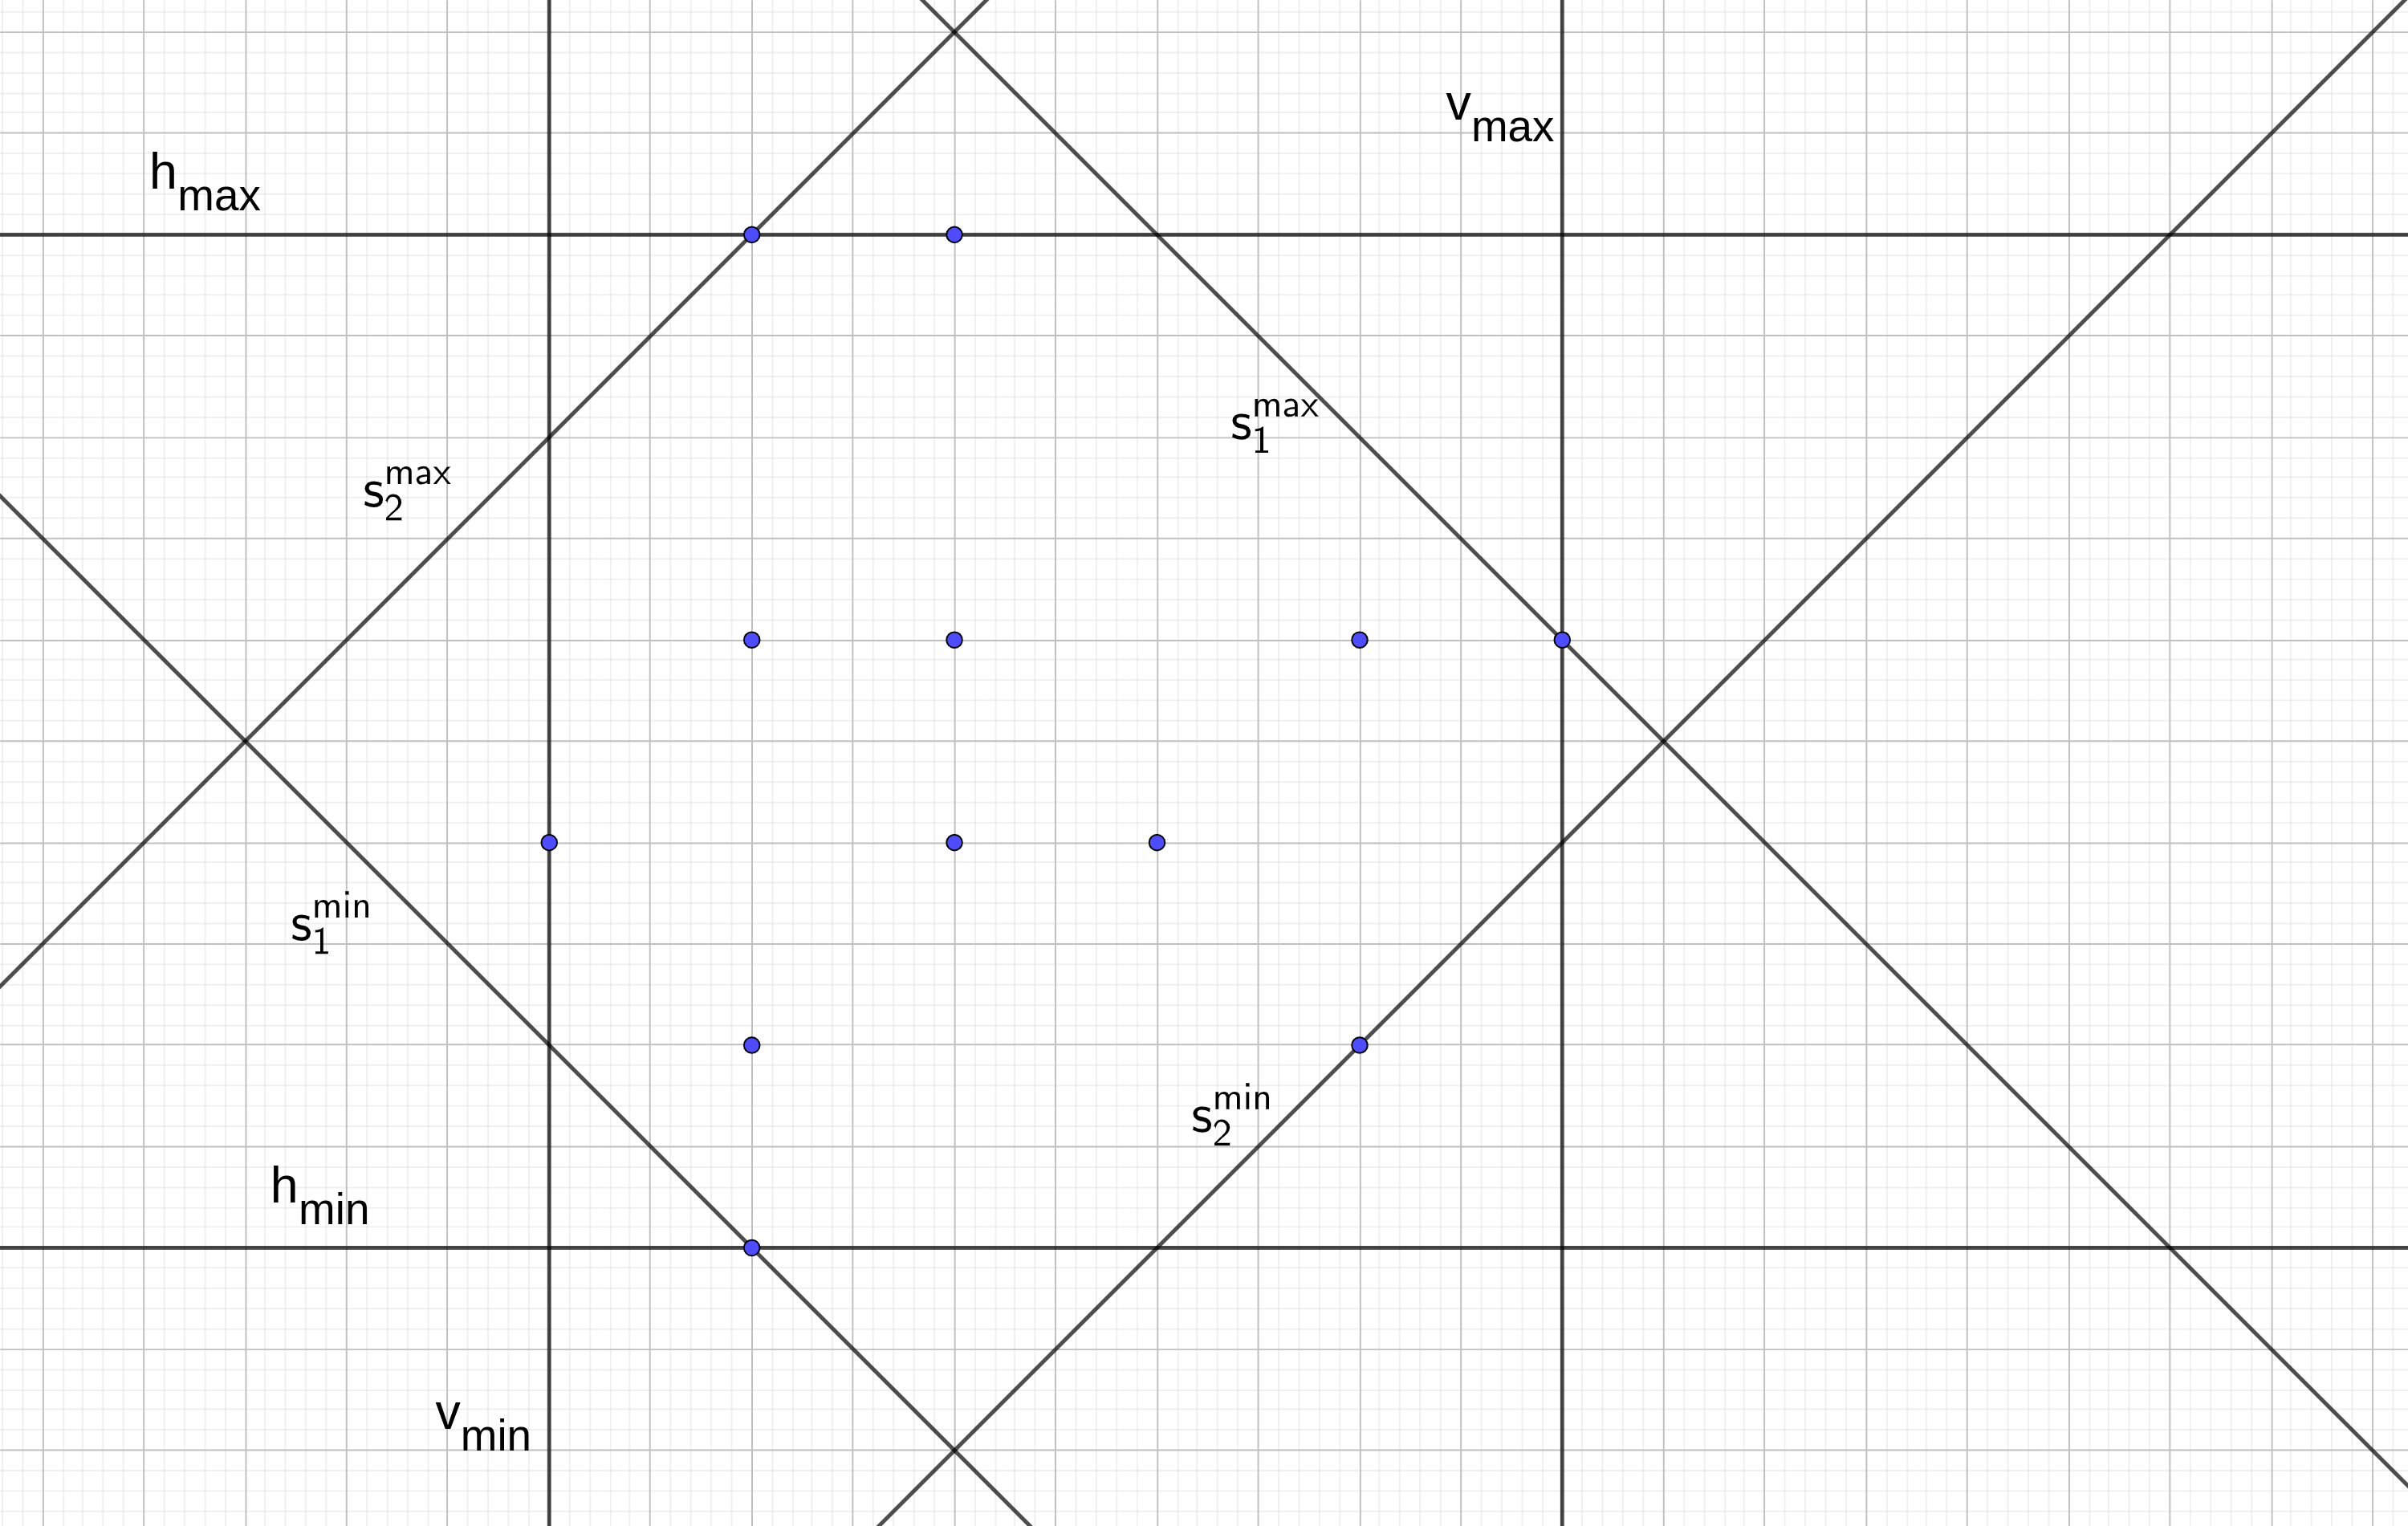
\includegraphics[scale = 0.8]{geogebra-export8.png}
    \end{figure}
    \item Βρίσκουμε τα σημεια:
            \begin{itemize}
                \item $\bf b_1$: σημείο τομής της $v_{min} $ με $s_2^{max}$  $\rightarrow O(1)$
                \item $\bf b_2$: σημείο τομής της $s_2^{max}$ με $h_{max} $  $\rightarrow O(1)$
                \item $\bf b_3$: σημείο τομής της $h_{max}$ με $s_1^{max} $  $\rightarrow O(1)$
                \item $\bf b_4$: σημείο τομής της $s_1^{max}$ με $v_{max} $  $\rightarrow O(1)$
                \item $\bf b_5$: σημείο τομής της $v_{max}$ με $s_2^{min} $  $\rightarrow O(1)$
                \item $\bf b_6$: σημείο τομής της $s_2^{min}$ με $h_{min} $  $\rightarrow O(1)$
                \item $\bf b_7$: σημείο τομής της $h_{min}$ με $s_1^{min} $  $\rightarrow O(1)$
                \item $\bf b_8$: σημείο τομής της $s_1^{min}$ με $v_{min} $  $\rightarrow O(1)$
            \end{itemize}
    \item Tο πολύγονο $[\bf b_1,b_2,b_3,b_4,b_5,b_6,b_7,b_8]$ είναι το ζητούμενο πολύγονο με την ελάχιστη περίμετρο που περιβάλει το σημεία του \textlatin{set} $P$. Σημειώνουμε οτι κάποια απο τα σημειά $\bf b_i$ μπορεί 
        να ταυτίζονται με τα γειτονικά τους
        \begin{figure}[H]

            \centering
            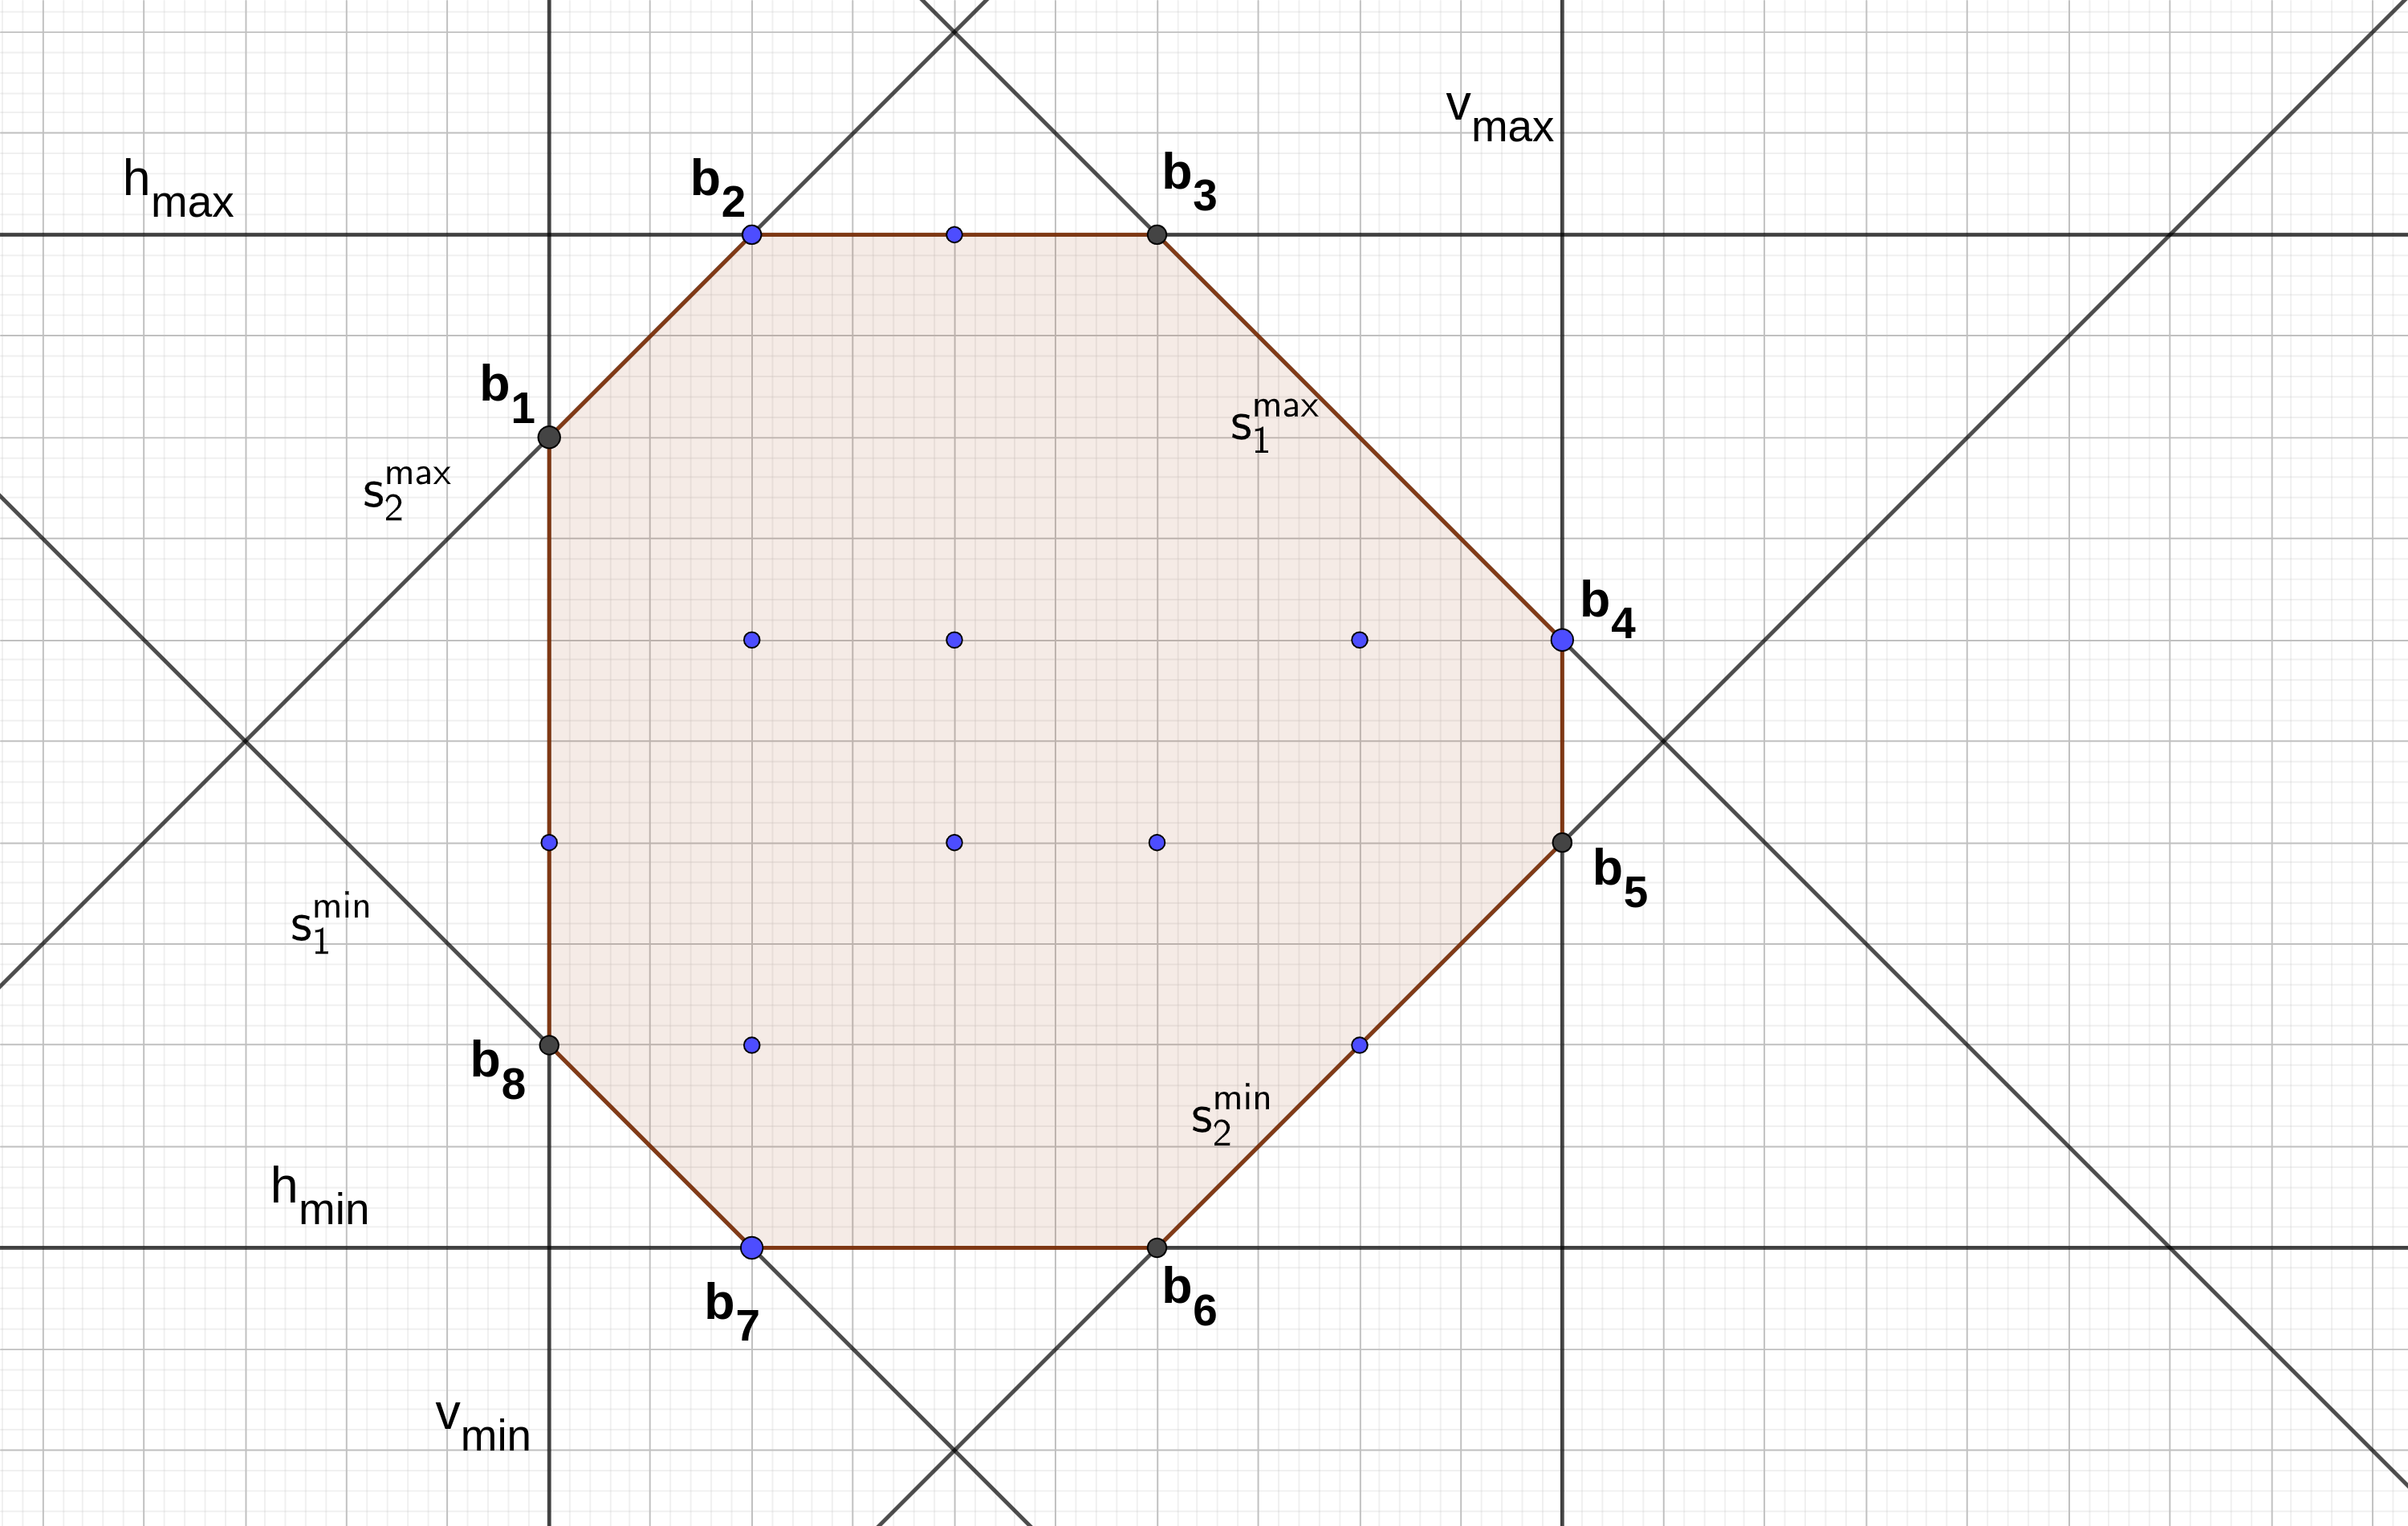
\includegraphics[scale = 1]{geogebra-export9.png}
        \end{figure}
    Η τελική πολυπλοκότητα του αλγορίθμου θα είναι 
    $$4O(n)+8O(1) = O(n)$$
    *Tα σημεία το παραδείγματος είναι τα ίδια με αυτά του παραδείγματος στην εκφώνηση της άσκησης
\end{enumerate} 
\rule{\textwidth}{.5pt}
\end{document}